
\documentclass[11pt,a4paper]{article}

\usepackage{amsmath,amsthm,mathtools}
\usepackage{booktabs,longtable,array,tabularx}
\usepackage{geometry}
\usepackage{natbib}
\usepackage{hyperref}
\usepackage{fontspec}
\usepackage{xeCJK}
\usepackage{unicode-math}
\usepackage{sectsty}
\usepackage{enumitem}
\usepackage{graphicx}
\usepackage{float}
\usepackage{xurl}
\usepackage{tikz}
\usetikzlibrary{positioning,arrows.meta,fit,shapes.multipart}

\geometry{top=20mm,bottom=20mm,left=22mm,right=22mm}
% Standard Japanese mathematical-paper typography:
% Japanese body text in Mincho, headings in Gothic, Latin text in Latin Modern,
% and all mathematical symbols in the dedicated Latin Modern Math font.
\setmainfont{Latin Modern Roman}
\setsansfont{Latin Modern Sans}
\setmonofont{Latin Modern Mono}
\setCJKmainfont[BoldFont=HaranoAjiMincho-Bold,ItalicFont=HaranoAjiMincho-Regular]{HaranoAjiMincho-Regular}
\setCJKsansfont[BoldFont=HaranoAjiGothic-Bold]{HaranoAjiGothic-Medium}
\setCJKmonofont{HaranoAjiGothic-Regular}
\setmathfont{Latin Modern Math}
\linespread{1.08}
\allsectionsfont{\sffamily\bfseries}
\XeTeXlinebreaklocale "ja"
\XeTeXlinebreakskip=0pt plus 1pt
\XeTeXlinebreakpenalty=0
\hypersetup{colorlinks=true,linkcolor=blue,citecolor=blue,urlcolor=blue,hypertexnames=false}
\renewcommand*{\theHtable}{\thesection.\arabic{table}}
\graphicspath{{figs/}}
\emergencystretch=2em
\setlength{\parskip}{2pt}
\raggedbottom
\numberwithin{equation}{section}
\numberwithin{table}{section}
\numberwithin{figure}{section}

\makeatletter
\renewcommand*\l@section{\@dottedtocline{1}{0em}{4.0em}}
\renewcommand*\l@subsection{\@dottedtocline{2}{1.8em}{4.8em}}
\makeatother

\theoremstyle{plain}
\newtheorem{theorem}{定理}
\newtheorem{proposition}{命題}
\newtheorem{lemma}{補題}
\newtheorem{corollary}{系}
\newtheorem{assumption}{仮定}

\theoremstyle{definition}
\newtheorem{definition}{定義}
\newtheorem{remark}{注意}
\renewcommand{\proofname}{証明}
\renewcommand{\abstractname}{要旨}
\renewcommand{\contentsname}{目次}
\renewcommand{\refname}{参考文献}
\renewcommand{\figurename}{図}
\renewcommand{\tablename}{表}

\newcommand{\E}{\mathbb{E}}
% Variables remain mathematical italics; named operators and differentials use
% the upright glyphs of the dedicated mathematics font.
\DeclareMathOperator{\Var}{Var}
\DeclareMathOperator{\Cov}{Cov}
\DeclareMathOperator{\CVaR}{CVaR}
\DeclareMathOperator{\VaR}{VaR}
\DeclareMathOperator{\Skew}{Skew}
\DeclareMathOperator{\Proj}{Proj}
\DeclareMathOperator{\Interp}{Interp}
\DeclareMathOperator*{\argmax}{arg\,max}
\DeclareMathOperator*{\argmin}{arg\,min}
\newcommand{\R}{\mathbb{R}}
\newcommand{\F}{\mathcal{F}}
\newcommand{\A}{\mathcal{A}}
\newcommand{\Lop}{\mathcal{L}}
\newcommand{\Hamil}{\mathcal{H}}
\newcommand{\dd}{\mathop{}\!\mathrm{d}}
\newcommand{\one}{\mathbf{1}}
\newcommand{\GH}{\mathrm{GH}}
\newcommand{\MC}{\mathrm{MC}}
\newcommand{\dt}{\Delta t}
\newcommand{\dx}{\Delta x}
\newcommand{\contribbox}[2]{%
\begin{minipage}[t]{0.48\textwidth}\small\textbf{#1}\par #2\end{minipage}}



\usepackage{pgfplots}
\usepgfplotslibrary{groupplots}
\pgfplotsset{compat=1.18}
\setlength{\textfloatsep}{12pt plus 2pt minus 2pt}
\setlength{\abovedisplayskip}{7pt plus 2pt minus 2pt}
\setlength{\belowdisplayskip}{7pt plus 2pt minus 2pt}
\setcounter{topnumber}{3}
\renewcommand{\topfraction}{.9}
\renewcommand{\textfraction}{.08}
\usepackage{placeins}
\setcounter{tocdepth}{1}
\title{確定拠出年金における制約付き動的平均--分散運用：\\\large 共通期待終価の比較，状態別退職成果と実装検証}
\author{第一生命保険株式会社\quad 永山義基}
\date{}
\begin{document}\maketitle
\begin{abstract}
確定拠出年金の運用では，将来拠出を含むリスク負担能力と，現在の口座で実行可能な投資額を区別する必要がある．また，平均--分散目的の時間非整合性により，初期計画へのコミットメント，逐次再計画，将来の自己との均衡は異なる方策を与える．本稿は継続拠出と空売り・借入禁止の下で，PCMV，DOMV，定数係数cTCMV，総年金富依存係数dTCMVを共通の枠組みで比較する．

理論面では，制約付き継続価値に基づく局所射影と無制約解の事後クリップを区別する．固定ターゲットの方策損失をBellman残差で表し，線形確率配分の追加分散を明示して，内部整合性と独立評価の役割を分ける．40年・月次の共通有限モデルで方策を再計算し，期待終価84.78へ再較正した．定率方策を含む5戦略の最大較正誤差は0.003547であり，独立100万経路による平均差の近似同時95\%区間は設定幅$\pm0.1$内に収まった．最適性・均衡性の直接の保証は有限モデル内に限定する．

再較正後のPCMVは標準偏差が最小である一方，下位5\%平均が最良ではない．他の戦略も，分位点，裾平均，不足確率により評価が異なる．さらに，新方策を三つの共通途中状態から各20万経路で評価し，総年金富依存方策の便益と費用が現在残高と残存期間に依存することを示す．退職所得への仮定上の換算により，数理的な差を加入者説明へ結びつける．特定方策の一律な推奨ではなく，目的，近似精度，退職成果を一貫して検証することを実務上の貢献とする．背景と導出，旧計算の監査，高次モーメント拡張を付録にまとめ，再現可能な図表・データを提供する．
\end{abstract}
\noindent\textbf{キーワード：} 確定拠出年金，時間非整合性，直接制約，平均--分散，ローリング評価，退職所得，数値検証．
\clearpage\tableofcontents\clearpage
\FloatBarrier
\section{序論}
\label{sec:introduction}
確定拠出年金（DC）の運用設計で重要なのは，配分曲線が滑らかであることだけではない．同じ年齢でも，現在残高，将来拠出，退職時の所得目標が異なれば，必要なリスク量も異なる．一方，モデルに基づく配分を実装する際には，投資制約を満たすことと，そのモデルの意思決定原理を再現することは別の要件である．

本稿の問いは，\emph{共通のDC制約の下で，異なる意思決定原理を同じ期待終価と現在状態から比較し，どの退職成果をどの精度で説明できるか}である．直接制約方策は，将来も制約に直面し得ることを継続価値へ織り込む．クリップ近似は，現在の投資額を実行可能にするが，将来の制約を無制約問題の継続価値へ反映しない．ただし，両者を数値的に比較した差には，方策の相違だけでなく，制御探索，残高補間，裾の打切りおよび較正の誤差も含まれ得る．

この問いを，PCMV（事前コミットメント），DOMV（逐次再最適化），cTCMV（定数係数の時間整合的均衡），dTCMV（富依存係数の時間整合的均衡）の四つについて扱う．四者は，同じ目的関数に対する競合アルゴリズムではない．時間を通じた意思決定原理と，リスクの評価方法が異なる運用仕様である．

本稿は，四解概念の比較と共通平均較正に\emph{独立した数値監査}を組み込む．後退計算と前進分布の一致は必要だが，両方が同じ補間誤差を共有すれば一致したまま成果を誤る．実際，公開参照版の定率運用に，解析的モーメントとの差が認められた．この診断を出発点として，旧計算の診断を付録\ref{sec:results}へ分離し，本文では再最適化・再較正した方策の結果を中心に論じる．

\subsection{ICAの五つの評価基準との対応}
ICA2026の論文作成指針は，関連性，品質，新規性，価値，将来性の五基準への配慮を求める\citep{ICA2026Guidance,ICA2026Call}．表\ref{tab:ica}は自己採点ではなく，読者が根拠を確認するための案内である．
\begin{table}[htbp]\centering\small
\caption{五つの評価基準と本稿の内容}\label{tab:ica}
\begin{tabularx}{\textwidth}{>{\raggedright\arraybackslash}p{31mm}X}
\toprule 観点 & 内容と確認箇所 \\ \midrule
関連性（Relevance） & 借入れを認めないDCで，簡便な配分を採用する前に何を検証すべきかを示す（第\ref{sec:model}，\ref{sec:practice}節）．\\
品質（Quality） & 導出，解析的モーメント，独立シミュレーション，数値残差を分けて検証する（第\ref{sec:cert}--\ref{sec:results}節）．\\
新規性（Originality） & 四解概念の実装比較に，補間分散・ターゲット離散化上界・共通平均較正の監査を結びつける（第\ref{sec:interpolation}，\ref{sec:equalmean}節）．\\
価値（Value） & 数理上の差を，下方所得，不足額および採用判断の説明へ変換する（第\ref{sec:rolling}，\ref{sec:practice}節）．\\
将来性（Future） & 再最適化・共通平均再較正を実施し，新方策の条件付き評価と裾の誤差を補足し，所得・長寿・取崩しへの拡張課題を示す（第\ref{sec:limits}節）．\\
\bottomrule\end{tabularx}\end{table}

\FloatBarrier
\section{DC運用の課題と先行研究における位置づけ}
\label{sec:background}
\subsection{残高の形成から退職所得の説明へ}
DCでは掛金が制度規則によって決まっていても，退職時の残高は投資収益率と拠出経路に依存する．加入者が必要とするのは，資産配分の形だけでなく，その配分が退職時の所得水準と不足の可能性をどのように変えるかという説明である．運用方策の評価では，期待値，分散，最低限の目標に届かない確率，届かなかった場合の不足額を区別する必要がある．同じ期待残高を持つ方策でも，これらの量は一致しない．

OECDの2025年報告は2024年の積立型年金を対象とし，職域DBの資産増加率4.0\%に対して職域DCは11.4\%と報告している\citep{OECD2025PensionMarkets}．この観測はDC運用の重要性を示す背景であるが，本稿の市場係数を推定するデータではない．国際統計における資産の範囲，対象国，観測年を区別し，資産規模の拡大そのものから特定の最適方策を導くことはしない．

DC運用の数理的な難しさには三つの側面がある．第一に，将来拠出は経済的なリスク負担能力に関係するが，口座内で直ちに投資できる資産ではない．第二に，平均--分散基準では，初期時点の望ましい計画と，将来の実現状態における望ましい計画が一致するとは限らない．第三に，制約付き方策を数値的に求める際，最適化の近似と成果評価の近似を同時に行うため，内部的には整合していても金融モデルに対する誤差が残り得る．

アクチュアリアルな貢献は，この三つを別々に分析するだけでなく，同じ加入者の意思決定へ接続することにある．どの状態でリスク資産比率が高くなるか，その理由が将来拠出なのか目標への不足なのか，期待成果の増加にどれだけの下方リスクが伴うかを説明する．モデルの複雑さは，説明の代わりにはならない．

\subsection{外生的グライドパスと状態依存フィードバック}
年齢だけで配分を定める方策を$g(t)$，年齢と現在残高で配分を定める方策を$g(t,x)$と書く．前者は同年齢の加入者に同じ配分を与え，後者は実現した積立状態に応じて配分を変える．状態依存方策の下で平均した曲線$\E[g(t,X_t)]$は一本のグライドパスに見えるが，各加入者に実際に適用される配分表そのものではない．

たとえば平均配分が年齢とともに低下しても，同じ年齢の低残高状態と高残高状態で大きな差があり得る．逆に，平均配分がU字型でも，すべての実現経路がU字型になるとは限らない．方策ヒートマップは$g(t,x)$を，平均グライドパスは到達分布で重み付けした要約を表す．本稿では両者を併記し，形状だけから運用原理を識別しない．

背景富を考慮するライフサイクル研究\citep{Merton1969,BodieMertonSamuelson1992,Viceira2001}と，拠出・退職目標を考慮するDC研究\citep{VignaHaberman2001,HabermanVigna2002,CairnsBlakeDowd2006}は，この区別を理解する基礎となる．本稿の追加的な焦点は，取引可能な口座残高と背景富を分けたまま，同じ制約と評価条件で異なる意思決定原理を比較する点にある．

\subsection{四解概念が答える異なる問い}
PCMVは，初期に選択した計画へコミットできる場合の効率性を表す．DOMVは，現在の状態から局所的に望ましい計画を選び直し，その現在成分を実行する．cTCMVとdTCMVは，将来の自己も各時点で判断することを認めた均衡である．これらを，計算速度や精度だけが異なる四つのアルゴリズムと扱うことはできない．

\begin{table}[htbp]\centering\small
\caption{先行研究と本稿の比較軸}\label{tab:literature-map}
\begin{tabularx}{\textwidth}{p{31mm}XX}\toprule
研究領域 & 既存の基礎 & 本稿で固定する比較軸\\\midrule
ライフサイクル配分 & 金融資産と背景富の関係 & 背景富を投資上限に算入しない\\
目標型DC & 拠出と退職目標を持つ動的運用 & 現在残高による両側投資制約\\
事前コミットメント & 二次損失への埋め込み & 同じ有限モデル内の達成平均と分散\\
動学的最適性 & 残存期間の計画の更新 & 計画上の成果と逐次実行成果の分離\\
時間整合的均衡 & 将来の自己に対する局所逸脱 & 定数係数と総年金富依存係数\\
終価分布比較 & 共通平均下の分位点・裾の比較 & 独立較正と条件付き退職成果\\
数値制御 & Markov近似・半Lagrange法 & 内部整合性と金融モデル精度の分離\\\bottomrule
\end{tabularx}
\end{table}

PCMVの埋め込み法は\citet{LiNg2000,ZhouLi2000}，DCへの平均--分散応用は\citet{Vigna2014,MenoncinVigna2017}に基礎を持つ．DOMVについては\citet{PedersenPeskir2017,MenoncinVigna2020}，均衡については\citet{BasakChabakauri2010,BjorkMurgociZhou2014,BjorkKhapkoMurgoci2017}を参照する．\citet{vanStadenDangForsyth2021}の共通平均下の終価分布比較に対して，本稿では継続拠出，DC残高による投資上限，独立評価と途中状態からの比較を明示する．表\ref{tab:literature-map}は論点の対応を示すものであり，先行研究の全定理を再検証した一覧ではない．

\subsection{本稿の貢献と読み方}
本稿の貢献は，既存の解概念を一つの最適性に還元することではない．第一に，直接制約問題とクリップ近似の差を，値関数・均衡モーメントに対する制約の内生化として整理する．第二に，固定ターゲットの方策損失と，補間の追加分散を別の量として把握する．第三に，共通期待終価への較正を独立評価で確認し，期待値以外の成果を比較する．第四に，同じ途中残高からの比較を退職所得へ翻訳する．

本文ではモデル，制御の定義，数値検証の原理，新較正の結果，途中状態の結果を順に示す．背景富・時間非整合性の補足，検証論証，アルゴリズムの詳細，旧計算の監査，高次モーメント拡張は付録に分離する．旧計算は誤差の発見と検証設計の理由を説明する資料であり，新方策の比較表と混合して順位を付けるための資料ではない．

ここでいう品質は，結果を強く言い切ることではなく，どの主張をどの式・データが支えるかを読者が追跡できることである．同様に，実務上の価値は複雑な方策への置換自体ではなく，加入者の成果に関する説明と選択の根拠を増やすことで評価する．
\FloatBarrier
\section{モデルと四つの意思決定原理}
\label{sec:model}
\subsection{拠出，投資制約と背景富}
有限期間$[0,T]$，通常の条件を満たすフィルトレーションとブラウン運動$B$を考える．安全資産の利率を$r$，リスク資産の期待収益率を$\mu$，ボラティリティを$\sigma>0$とし，$\beta=\mu-r>0$と置く．DC残高$X$と投資額$\pi$は
\begin{equation}
\dd X_t=(rX_t+c_t+\beta\pi_t)\dd t+\sigma\pi_t\dd B_t,
\quad X_0=x_0\geq0,\quad 0\leq\pi_t\leq X_t
\label{eq:state}
\end{equation}
を満たす．$c_t\geq0$は有界連続な確定的拠出である．この制約は本稿の運用モデルの仕様であり，各国のすべてのDC商品の法的制約を表すものではない．

許容制御は，$[0,1]$値の進行可測な比率過程$u$により$\pi_t=u_tX_t$と表す．固定された過程$u$について状態方程式は線形成長・Lipschitz条件を満たし，一意な強解を持つ．$x=0$でも拠出があれば吸収状態ではない．比率$\pi/x$は$x>0$で定義し，$x=0$での便宜的な値を経済的な配分判断と解釈しない．閉ループの可測フィードバックについては，別途，状態方程式の適切性が必要である．

退職時に受け取る確定額$D_T\geq0$と将来拠出の現在価値を
\begin{equation}
H_t=\int_t^T e^{-r(s-t)}c_s\dd s+e^{-r(T-t)}D_T,
\qquad \dot H_t=rH_t-c_t,
\label{eq:H}
\end{equation}
とする．$Y_t=X_t+H_t$と置くと
\begin{equation}
\dd Y_t=(rY_t+\beta\pi_t)\dd t+\sigma\pi_t\dd B_t,
\qquad Y_T=X_T+D_T=:W_T.
\label{eq:Y}
\end{equation}
$Y$は評価上の総年金富であり，すべてが取引可能な資産ではない．投資上限は$Y$ではなく$X$である．$D_T$を終身年金の給付流列と解釈するには，退職時点の年金現価へ変換する必要があり，確率的な年金化価格や長寿リスクは本モデルには含まれない．

\subsection{解概念と係数の単位}
\begin{table}[htbp]\centering\small
\caption{四つの解概念}\label{tab:concepts}
\begin{tabularx}{\textwidth}{p{17mm}X p{39mm}}
\toprule 解概念 & 意思決定原理 & 主要入力 \\ \midrule
PCMV & 初期に選んだ平均--分散戦略に満期まで従う． & $\gamma_p$，または固定ターゲット$m$ \\
DOMV & 各状態で残存期間問題を解き直し，現在成分だけを採用する． & $\gamma_D=2\lambda_D$ \\
cTCMV & 将来の自己の方策を所与として短時間逸脱を評価する均衡． & 定数$\gamma_c$ \\
dTCMV & 同じ均衡概念で，現在の総年金富に応じた係数を用いる． & $\Gamma(t,x)=\rho_d/(x+H_t)$ \\
\bottomrule\end{tabularx}\end{table}
平均--分散の目的は$\E[W_T]-(\gamma/2)\Var(W_T)$である．$\gamma$の単位は金額の逆数，$\rho_d$は無次元であり，係数の数値だけから戦略間のリスク許容度を比較できない．金額の単位を$k$倍に変更すると，定数係数は$\gamma/k$に変換する．dTCMVの$\rho_d$を固定すれば，同時に拠出，残高，背景富を$k$倍する尺度変更と整合する．

dTCMVは$x+H_t>0$の領域で定義する．$x+H_t=0$では，非負の拠出と給付という仮定の下で，将来の資金もなく投資額はゼロに限られる．この退化状態では$J=0$，$\pi=0$と別定義する．$T$には新たな投資判断を置かず，$\Gamma(T,0)$を計算する必要はない．

確定額$D_T$の加算は分散を変えない．PCMV・DOMV・cTCMVでは定数係数を固定する限り，$D_T$は目的の加算定数となる．固定ターゲット問題では$m$を$D_T$だけ平行移動する必要がある．一方，dTCMVでは$D_T$が$\Gamma$を変えるため，運用へ影響する．これは背景富に関する\emph{選好の仮定}の結果であり，大きなDB給付がある人は必ずリスクを好むという実証結果ではない．

\FloatBarrier
\section{直接制約方策とクリップ近似}
\label{sec:theory}
\subsection{PCMVとDOMV}
固定ターゲット$m$の二次損失値関数を
\begin{equation}
L^m(t,x)=\inf_{\pi\in\mathcal A_{t,x}}\E_{t,x}[(W_T-m)^2]
\label{eq:loss}
\end{equation}
とする．生成作用素$\mathcal L^\pi f=(rx+c_t+\beta\pi)f_x+\tfrac12\sigma^2\pi^2f_{xx}$により，対応するHJBは
\begin{equation}
L_t^m+\inf_{0\leq\pi\leq x}\mathcal L^\pi L^m=0,
\qquad L^m(T,x)=(x+D_T-m)^2.
\label{eq:hjb}
\end{equation}
十分な正則性，$L_{xx}^m>0$および閉ループの適切性が成り立てば，最適投資額は
\begin{equation}
\pi^{m,*}(t,x)=\Proj_{[0,x]}\left(-\frac{\beta L_x^m}{\sigma^2L_{xx}^m}\right).
\label{eq:pcproj}
\end{equation}
このターゲット方策が$\E[W_T]=d$を満たせば，同じ平均$d$を持つ方策の中で分散を最小化する．なぜなら，平均$d$の下では$\E[(W_T-m)^2]=\Var(W_T)+(d-m)^2$だからである．任意の$d$の達成可能性は別途確認する．

スカラー化MV問題では，任意の許容方策の平均を$a$とすると
\begin{align}
m-\frac1{2\gamma}-\frac\gamma2\E[(W_T-m)^2]
&=a-\frac\gamma2\Var(W_T)-\frac\gamma2\left(m-a-\frac1\gamma\right)^2,\label{eq:envelope-id}\\
\sup_\pi J_\gamma(t,x;\pi)
&=\sup_{m\in\mathbb R}\left\{m-\frac1{2\gamma}-\frac\gamma2L^m(t,x)\right\}.
\label{eq:envelope}
\end{align}
PCMVは時点0で外側ターゲットを選び固定する．DOMVは各$(t,x)$で同じ外側最大化を行い，選んだ固定ターゲット問題の現在成分を採用する．固定点$m=a+1/\gamma$を満たすだけでは大域的最大化を証明しない．DOMVの計画上の継続平均と，次時点以降も再最適化する実行方策の継続平均も区別する．

\subsection{時間整合的均衡}
候補フィードバック$\hat\pi$が均衡であるとは，許容逸脱$\nu$を$[t,t+h)$だけ使って元の方策へ戻すとき
\begin{equation}
\liminf_{h\downarrow0}\frac{J(t,x;\hat\pi)-J(t,x;\nu\otimes_h\hat\pi)}h\geq0
\label{eq:eqdef}
\end{equation}
となることである．これは一次の局所均衡であり，任意の有限期間の逸脱に対する大域最適性ではない．

候補方策の条件付きモーメント$F=\E[W_T]$，$G=\E[W_T^2]$は
\begin{equation}
F_t+\mathcal L^{\hat\pi}F=0,\quad G_t+\mathcal L^{\hat\pi}G=0,
\quad F(T,x)=x+D_T,\quad G(T,x)=(x+D_T)^2
\label{eq:FG}
\end{equation}
を満たす．逸脱評価中は現在の自己の$\Gamma(t,x)$を固定し，
\begin{align}
\mathcal H(t,x,\pi)&=(1+\Gamma F)(F_t+\mathcal L^\pi F)-\frac\Gamma2(G_t+\mathcal L^\pi G),\label{eq:ham}\\
A_F&=(1+\Gamma F)F_x-\frac\Gamma2G_x,\qquad
B_F=(1+\Gamma F)F_{xx}-\frac\Gamma2G_{xx}
\label{eq:AB}
\end{align}
と置く．$B_F<0$なら
\begin{equation}
\hat\pi=\Proj_{[0,x]}\left(-\frac{\beta A_F}{\sigma^2B_F}\right).
\label{eq:eqproj}
\end{equation}
$\Gamma$が定数のcTCMVでは，$V=F-\tfrac\Gamma2(G-F^2)$を用い$A_F=V_x$，$B_F=V_{xx}-\Gamma F_x^2$となる．dTCMVでは$V$の全微分に$\Gamma_x$が入るため，これをそのまま局所目的の微分へ代入してはならない．式\eqref{eq:ham}は現在の係数を固定する均衡定義と整合する\citep{BjorkMurgociZhou2014,BjorkKhapkoMurgoci2017}．

正則性，モーメント表示と閉ループの適切性の下で，式\eqref{eq:ham}を各点で最大化する方策は式\eqref{eq:eqdef}を満たす（付録\ref{app:verify}）．$B_F=0$では線形目的の端点比較，$B_F>0$では凸二次式の端点比較を用い，射影公式を適用しない．$x=0$では許容投資額は一つだけであり，下限・上限領域を重複させて自由境界と呼ばない．状態依存両側制約の下での大域的均衡の存在・一意性は，本稿の検証定理からは従わない．

\subsection{無制約ベンチマークと符号の確認}
\label{sec:theta}
$A=\beta^2/\sigma^2$，$y=x+H_t$と置く．無制約解の投資額は
\begin{align}
\pi^{p,0}(t,y;m)&=\frac\beta{\sigma^2}(me^{-r(T-t)}-y),\label{eq:uncp}\\
\pi^{D,0}(t,y)&=\frac\beta{\gamma_D\sigma^2}e^{(A-r)(T-t)},\label{eq:uncD}\\
\pi^{c,0}(t,y)&=\frac\beta{\gamma_c\sigma^2}e^{-r(T-t)},\label{eq:uncc}\\
\pi^{d,0}(t,y)&=\theta(t)y.
\label{eq:uncd}
\end{align}
PCMVの固定ターゲット比較では両方策で$m$を一致させる．スカラー化比較では$\gamma_p$を一致させた上で各問題のターゲットを選ぶ．この二つの設計を混同しない．

dTCMVについて，無制約方策$\pi=\theta(t)y$のモーメントを$F=a(t)y$，$G=b(t)y^2$と書くと
\begin{equation}
a(t)=e^{\int_t^T(r+\beta\theta_s)\dd s},\qquad
b(t)=e^{\int_t^T\{2r+2\beta\theta_s+\sigma^2\theta_s^2\}\dd s}.
\label{eq:abtheta}
\end{equation}
式\eqref{eq:AB}--\eqref{eq:eqproj}から
\begin{align}
\theta(t)&=\frac\beta{\rho_d\sigma^2}\left\{\frac{a(t)}{b(t)}+
\rho_d\frac{a(t)^2}{b(t)}-\rho_d\right\}\label{eq:thetamon}\\
&=\frac\beta{\rho_d\sigma^2}\left\{
e^{-\int_t^T(r+\beta\theta_s+\sigma^2\theta_s^2)\dd s}
+\rho_d e^{-\int_t^T\sigma^2\theta_s^2\dd s}-\rho_d\right\}.
\label{eq:thetacorrect}
\end{align}
第一指数の被積分関数の分散項は\textbf{$+\sigma^2\theta_s^2$}である．これは\citet{BjorkMurgociZhou2014}の原論文の式(13)--(15)と整合する．\citet{vanStadenDangForsyth2021}の式(3.5)ではこの項が負号で表示され，参照実装もその表示を使用していた．本稿は式\eqref{eq:abtheta}の二次モーメントと一階条件に基づき，式\eqref{eq:thetacorrect}を採用する．文献の他の結果をこの一点だけから否定するものではない．

クリップ近似を$\pi^{j,\mathrm{clip}}=\Proj_{[0,x]}\{\pi^{j,0}(t,x+H_t)\}$と定める．式\eqref{eq:pcproj}や\eqref{eq:eqproj}の射影中心は\emph{制約付き}継続価値から得るため，無制約解をクリップする操作とは一般に異なる．十分条件として，無制約方策が将来を含む関連状態で実行可能であり，対応する検証条件を満たせば一致する．一点で上限・下限が一致することだけから，全方策の同一性は結論できない．

\FloatBarrier
\section{方策差を検証可能な量へ変える}
\label{sec:cert}
\subsection{固定ターゲットの方策損失とBellman残差}
共通の有限状態Markovモデルを固定し，$P_n^u$を行和1の非負遷移行列とする．終端損失$\ell_i=(x_i+D_T-m)^2$に対して，離散最適値$L_n$は
\begin{equation}
L_N=\ell,\qquad L_n(i)=\min_u(P_n^uL_{n+1})(i)
\label{eq:discreteBellman}
\end{equation}
を満たす．方策$b$の残差を$R_n^b=P_n^bL_{n+1}-L_n\geq0$とする．
\begin{proposition}[離散方策損失の表示]
初期分布$p_0$から方策$b$で生成した到達分布を$p_n^b$とすると，
\begin{equation}
\E_b[\ell(X_N)]-p_0L_0=\sum_{n=0}^{N-1}p_n^b R_n^b.
\label{eq:bellmangap}
\end{equation}
\end{proposition}
\begin{proof}
$p_{n+1}^b=p_n^bP_n^b$より，$p_n^bR_n^b=p_{n+1}^bL_{n+1}-p_n^bL_n$である．時間について和を取ると中間項が相殺する．
\end{proof}
この標準的な恒等式をクリップ監査に使えば，「平均比率が近い」という記述を，固定ターゲット損失の差へ変換できる．実用上は数値候補$\widetilde L$しかない場合も多い．$\widetilde L_N=\ell$，$e_n=\widetilde L_n-\min_uP_n^u\widetilde L_{n+1}$とし，$b$が$\widetilde L$に対して貪欲なら
\begin{equation}
0\leq J_b-L_0^*\leq2\sum_n\|e_n\|_\infty
\label{eq:resbound}
\end{equation}
という有限モデル内の誤差保証を得る．遷移作用素の最大値ノルムでの非拡大性と後退帰納法を用いる．クリップを評価する場合には，貪欲方策との一段階目的差も加える必要がある．これらの保証は，ターゲット不一致，別の遷移核，連続時間離散化の誤差を自動的には含まない．

PCMVの平均と分散のどちらが良いかを論じる際にも目的を固定する．固定$m$の損失最小性から，平均が異なる二方策の分散順位は導けない．DOMVとTCMVでは，それぞれ局所計画と一期間逸脱を評価するため，時点0のMV差を一律の「最適化損失」と呼ばない．

\subsection{配分差と成果差を区別する}
同じ状態での比率差$|g^{\mathrm{dir}}_n(x)-g^{\mathrm{clip}}_n(x)|$と，各方策自身の残高分布で平均した比率の差は異なる．後者は
\begin{equation}
G_{\mathrm{MAE}}=\frac1N\sum_n\left|\E_{\mathrm{dir}}[g_n(X_n)]-
\E_{\mathrm{clip}}[g_n(X_n)]\right|
\label{eq:gmae}
\end{equation}
である．異なる状態の誤差が相殺し得るので，$G_{\mathrm{MAE}}$が小さくても，局所方策や裾指標の一致は保証されない．成果指標を直接確認する必要がある．

\FloatBarrier
\section{数値実装と独立監査}
\label{sec:interpolation}
\subsection{月次Eulerモデルと格子モデル}
月次の近似遷移を
\begin{equation}
\widehat X_{n+1}=x+(rx+c_n+\beta\pi)\Delta t+
\sigma\pi\sqrt{\Delta t}\,Z_n,\qquad Z_n\sim N(0,1)
\label{eq:euler}
\end{equation}
とする．これは連続時間拠出・運用のEuler近似である．月次に意思決定するという事実だけで，Euler近似が実際の月次売買を厳密に表すわけではない．正規遷移には負残高の可能性があり，ゼロへの切上げは元のSDEとは別の数値処理である．本稿の独立シミュレーションでは切上げ発生数も記録する．

Gauss--Hermite（GH）求積では，標準正規に合わせた節点$\xi_k$と正の重み$w_k$（$\sum_kw_k=1$）を使う．候補点$z$が隣接残高$x_\ell,x_{\ell+1}$の間にあるとき，線形補間は，$z$を両端に確率配分する操作と同じである．
\begin{proposition}[線形配分による追加分散]
\label{prop:interpolation}
$x_\ell\leq z\leq x_{\ell+1}$とし，$\widetilde z$を平均$z$となるように両端点へ配分する．このとき
\begin{equation}
\E[\widetilde z\mid z]=z,\qquad
\Var(\widetilde z\mid z)=(z-x_\ell)(x_{\ell+1}-z)
\leq\frac{(x_{\ell+1}-x_\ell)^2}{4}.
\label{eq:interpvar}
\end{equation}
\end{proposition}
\begin{proof}
上端の重みを$q=(z-x_\ell)/(x_{\ell+1}-x_\ell)$と置く．平均は$z$，分散は$q(1-q)(x_{\ell+1}-x_\ell)^2$となる．
\end{proof}
したがって，境界処理前の同じ候補点分布について
\begin{equation}
\Var(\widetilde X_{n+1}\mid X_n)
=\Var(\widehat X_{n+1}\mid X_n)+
\E[(\widehat X_{n+1}-x_\ell)(x_{\ell+1}-\widehat X_{n+1})\mid X_n].
\label{eq:artificial}
\end{equation}
前進分布と後退モーメントを同じ線形配分で計算すれば，この追加分散を\emph{両方とも}含んだまま一致する．上端集約は反対に右裾を圧縮するため，最終的な誤差の符号は追加分散だけでは決まらない．状態依存方策では，変わった残高が次の制御も変える．

連続時間近似の整合性を議論する場合，局所的な補間誤差を$\Delta t$で除した影響も確認する．例えば滑らかな関数に対する十分な局所条件は，対象領域の最大格子幅$h_x$について$h_x^2/\Delta t\to0$である．時間格子だけを細分化して状態格子を固定する検証は不十分となり得る．これは本稿の非線形均衡系に対する包括的収束定理ではない．

\subsection{区分線形補間の下での制御探索}
現在状態を固定すると，各GH候補点は制御$u\in[0,1]$のアフィン関数$z_k(u)=a_k+b_ku$である．候補点が残高格子点を通過するすべての$u$と$0,1$を集め，重複を除いた集合を$\mathcal B$とする．一定値の境界集約を用いる場合，その切替点も含める．
\begin{proposition}[有限モデルの一段階大域探索]
\label{prop:breakpoints}
線形補間と有限GH求積の下で，固定ターゲットの一段階二次損失最小化には$\mathcal B$上の最小点が存在する．MV均衡の一段階目的
\begin{equation}
\Psi(u)=M(u)-\frac\Gamma2\{Q(u)-M(u)^2\},\qquad\Gamma>0
\label{eq:psidiscrete}
\end{equation}
にも$\mathcal B$上の最大点が存在する．
\end{proposition}
\begin{proof}
隣接する切替点の間では，補間された期待損失，$M$，$Q$はすべて$u$のアフィン関数である．損失最小値は区間端点で達成できる．また$M(u)=m_0+m_1u$なら$\Psi''(u)=\Gamma m_1^2\geq0$なので，最大値も区間端点で達成できる．有限個の区間を比較すればよい．
\end{proof}
連続HJBの局所ハミルトニアンが凹二次式であっても，線形補間後の一段階目的全体の凹性は保証されない．粗い制御格子の最良点の周囲を放物線補間するだけでは，大域的な一期間均衡を証明できない．本稿の\path{breakpoint_audit.py}は，保存済み方策の継続モーメントを同一の境界集約モデルで評価し，この有限候補集合との逸脱差を計算する．この監査は再最適化ではなく，一段階残差の検出である．

\subsection{定率運用による解析的な監査}
\label{sec:cp}
CPは$\pi=\theta_{cp}X$を用いる．$a=r+\beta\theta_{cp}$，$v=\sigma^2\theta_{cp}^2$，$A_h=1+a\Delta t$とし，$m_n=\E[X_n]$，$q_n=\E[X_n^2]$とすると，格子配分と境界切上げのないEuler遷移のモーメントは厳密に
\begin{align}
m_{n+1}&=A_hm_n+c\Delta t,\label{eq:cpm}\\
q_{n+1}&=(A_h^2+v\Delta t)q_n+2A_hc\Delta t\,m_n+c^2\Delta t^2
\label{eq:cpq}
\end{align}
を満たす．これは独立な市場ショックの一次・二次モーメントだけを用い，2点以上の正規化GHショックにも成り立つ．連続時間では$m'=am+c$，$q'=(2a+v)q+2cm$となる．後者を解けば，Euler時間近似の影響と残高格子配分の影響を分けて点検できる．

\FloatBarrier
\section{共通期待終価への再最適化と再較正}
\label{sec:equalmean}
\subsection{比較を成立させる計算仕様}
旧計算の保存方策監査を受け，四つの意思決定原理に従って方策を新たに計算し，共通期待終価$m_*=84.78$へ再較正した．以下は保存方策の係数だけを事後的に置換した結果ではない．PCMVでは固定ターゲット問題を解き直し，cTCMV・dTCMVでは継続モーメントを後退更新する均衡計算を各係数について実行した．DOMVでは固定ターゲット方策群を再計算し，各時点・各残高で埋め込みスコアを比較して第一期の投資額を選び直した．

全戦略に月次Euler遷移，$[0,600]$の残高範囲，非負の線形確率配分，上端集約を共通に適用する．基準計算は残高刻み0.2，65個の投資比率，5点GH，精緻化計算は残高刻み0.1，129個の投資比率，7点GHである．各格子状態では投資比率$\{j/128:j=0,\ldots,128\}$をすべて比較する．この全数探索は\emph{有限制御集合上}の大域探索であり，連続制御全体に対する大域最適性の証明とは区別する．

較正用評価では，投資額の補間と残高の遷移を分け，より細かい残高刻み0.025と31点GHを用いる．初期残高は正確に$x_0=1/12$から遷移させる．さらに独立した正規乱数を用い，残高を格子へ配分せず，上端で打ち切らないシミュレーションで評価する．較正値そのものと，独立標本で観測される平均の違いを表中に分けて示す．

係数探索では各試行で方策を再計算し，目標平均との差が最も小さい試行を保存する．有限制御集合の均衡選択は係数に対して不連続となり得るため，二分探索の使用を単調性・解の存在の証明とはしない．探索の終了だけで成功とせず，最終較正誤差0.01以内という条件を保存方策の再評価で検査する．独立評価には，全10組の平均差についてBonferroni補正した近似同時95\%信頼区間を用い，すべてが$(-0.1,0.1)$に入ることを別の実用上の同等性基準とする．これらは数値・統計上の許容差であり，実数としての厳密な同一平均を主張するものではない．

\subsection{PCMVとDOMVの最適性の確認範囲}
\begin{proposition}[固定ターゲットと共通平均]
固定ターゲット$z$について$\pi^z$が$\E[(W_T-z)^2]$を最小化するとする．その平均を$m_z$とすると，$\pi^z$は$\E[W_T]=m_z$を満たす同じ許容集合の方策の中で終価分散を最小化する．
\end{proposition}
\begin{proof}
平均$m_z$を固定すれば，$\E[(W_T-z)^2]=\Var(W_T)+(m_z-z)^2$の第二項はすべての比較方策で同じである．
\end{proof}
本計算ではこの論証が直接保証するのは，構成した有限モデル内で達成される平均に対する分散最小性である．独立評価モデルで84.78へ較正した結果を，連続時間問題の厳密な効率的フロンティアと同一視しない．

\begin{proposition}[DOMVのターゲット離散化誤差]
有限モデルで$0\leq W_T\leq L$，$\gamma>0$とする．固定ターゲット問題を正確に解き，$[0,L+1/\gamma]$を最大間隔$\delta$のターゲット集合で覆うとき，埋め込みスコアの大域最大値の不足は$\gamma\delta^2/8$以下である．
\end{proposition}
\begin{proof}
任意の方策の平均を$m$とすると，その埋め込みスコアは$z=m+1/\gamma$で最大となり，最大値からの差は$\gamma(z-m-1/\gamma)^2/2$である．最適方策の最大点から距離$\delta/2$以内のターゲットを選び，そのターゲットでも方策を最適化すれば，主張の上界を得る．
\end{proof}
本計算のDOMV較正範囲は$0.02\leq\gamma\leq0.2$であり，$L=600$に対してターゲット$0,2,\ldots,650$をすべて比較する．最適ターゲットの範囲を包含することと，選択されたターゲットが境界へ張り付いていないことを別々に確認する．上の誤差は各状態の\emph{事前コミットメント問題の埋め込み値}の誤差であり，逐次実行するDOMVの最終分布の誤差上界ではない．

\begin{table}[htbp]\centering\small
\caption{共通期待終価84.78への再較正（精緻化計算）}\label{tab:recalibration}
\begin{tabular}{lrrr}\toprule 方策 & 較正パラメータ & 較正用の平均 & 目標との差 \\ \midrule
PCMV & 101.35742188 & 84.78139 & +0.00139 \\
DOMV & 0.08624756 & 84.78159 & +0.00159 \\
cTCMV & 0.05411865 & 84.78355 & +0.00355 \\
dTCMV & 1.61425781 & 84.77719 & -0.00281 \\
CP & 0.46888422 & 84.78000 & -0.00000 \\
\bottomrule\end{tabular}
\par\vspace{3pt}\begin{minipage}{.96\textwidth}\footnotesize PCMVはターゲット$z$，DOMV・cTCMVは定数係数$\gamma$，dTCMVは$\rho$，CPは定率比率を較正する．CPの平均はEulerモーメント再帰による解析値．他の方策は再最適化した投資額を別の細かい格子で評価した値である．\end{minipage}\end{table}
\begin{table}[htbp]\centering\small
\caption{再最適化・再較正後の独立正規Euler評価（100万経路）}\label{tab:equalmeanmc}
\begin{tabular}{lrrrrrr}\toprule 方策 & 平均 & SE & 標準偏差 & 下位5\%点 & LCVaR$_{5\%}$ & $\Pr(W_T<60)$ \\ \midrule
PCMV & 84.772 & 0.019 & 18.942 & 38.194 & 28.799 & 0.117 \\
DOMV & 84.783 & 0.024 & 24.414 & 46.869 & 39.204 & 0.155 \\
cTCMV & 84.791 & 0.023 & 23.157 & 47.161 & 38.527 & 0.143 \\
dTCMV & 84.786 & 0.032 & 32.313 & 43.173 & 37.332 & 0.226 \\
CP & 84.785 & 0.032 & 31.687 & 45.227 & 39.900 & 0.214 \\
\bottomrule\end{tabular}
\par\vspace{3pt}\begin{minipage}{.96\textwidth}\footnotesize 全方策に同じ正規ショックを与える．Numbaのブロック別乱数を用い，seedは$20260912+1009b$（$b=0,\ldots,99$），各ブロック1万経路である．較正後の方策を固定して実行した検証標本であり，この標本に平均を事後的に合わせていない．上端打切り・格子への残高配分は行わない．\end{minipage}\end{table}


\subsection{独立評価，収束および解釈}
独立評価の平均は標本誤差を伴うため，小数点以下を強制的に一致させて表示しない．平均差について共通乱数による対応のある標準誤差と95\%信頼区間を併記した機械可読データを公開する．同じ期待終価という条件は，較正用の数値許容差と独立評価の不確実性を伴う条件として扱う．

PCMVは終価分散を小さくする一方，下位5\%点や下位裾平均まで最大にするわけではない．平均--分散，目標不足確率，下位裾平均は異なる評価基準である．また，DOMV・cTCMV・dTCMVはPCMVと同じ目的関数の解法違いではなく，継続時の意思決定原理・選好が異なる．従って，標準偏差の順序だけから制度全体の推奨方策を一意に決めることはできない．

補間による追加分散は精緻化後もゼロではない．較正したCP比率に対する解析的標準偏差は31.673923であり，評価格子刻み0.2，0.1，0.05，0.025の値はそれぞれ約32.025，31.745，31.693，31.679となる．独立Monte Carlo，格子の精緻化，GH次数の変更を別々に確認する理由がここにある．途中の9点GH評価では均衡方策の平均に約0.06のずれが残ったため，最終較正は31点へ増やしてやり直した．

一段階連続制御の補助監査では，各補間区間の全境界と端点を比較する．これは選択した時点・残高における厳密な一次元探索であり，全状態空間の誤差上界とは称さない．前進・後退モーメントの一致は有限モデルの実装検証とし，独立評価の精度保証から分離する．上端600から900への変更，残高・制御格子および求積次数の感応度は同梱データに記録する．
上端を900へ拡大し同じ係数で再最適化すると，dTCMVの平均は84.777から84.703へ変化した．したがって，上端到達が標本で観測されないことだけで境界の無影響を結論しない．拡大モデルで$\rho=1.61457031$へ再較正すると平均84.778，標準偏差32.287となり，上端600での同じ平均の評価値32.300に近づいた．この比較は境界変更時の再較正の必要性を示す感応度検査であり，全境界・全均衡分枝に対する収束証明ではない．







\begin{figure}[htbp]\centering
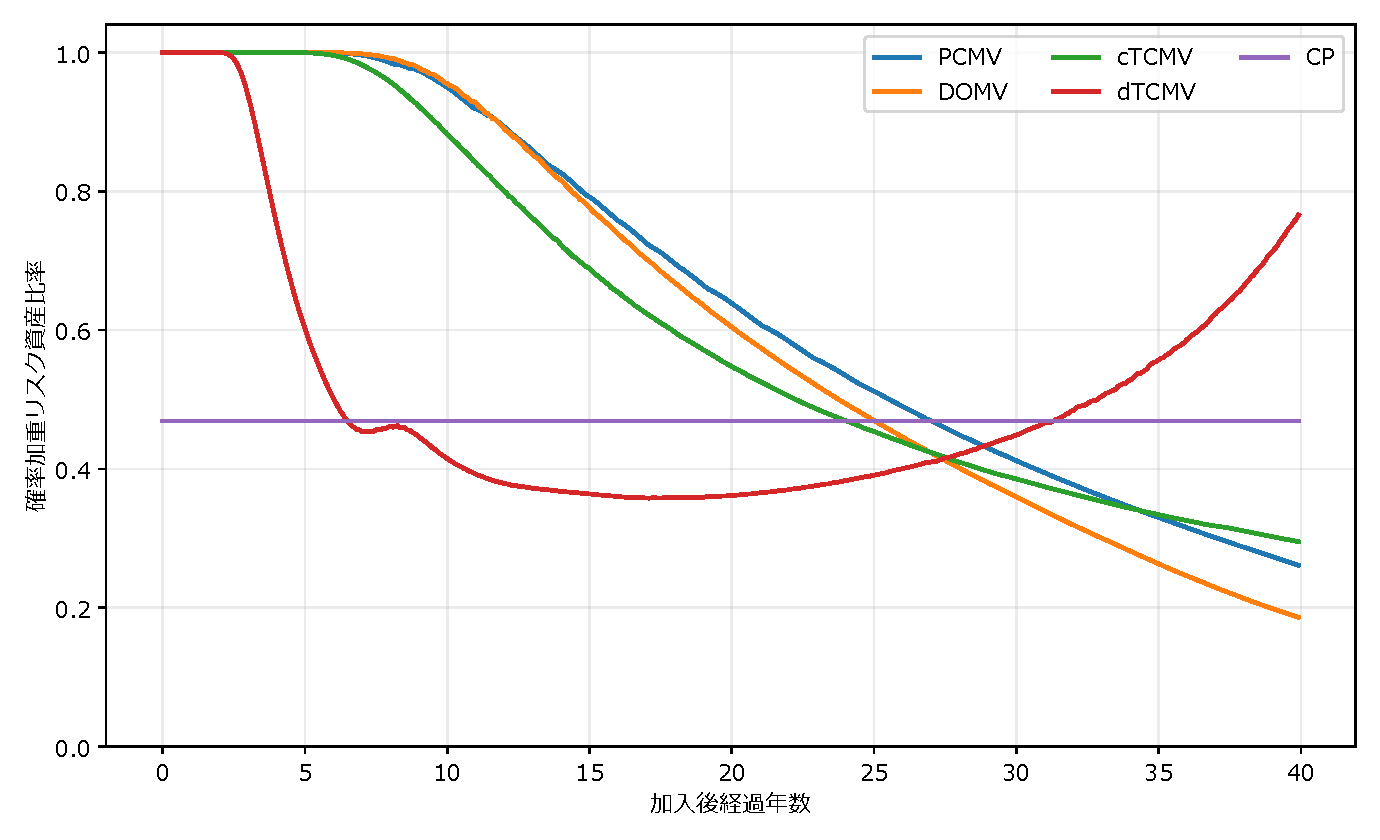
\includegraphics[width=.94\textwidth]{glidepaths_v9.pdf}
\caption{共通期待終価へ再較正した5戦略の平均配分．v8方策の独立100万経路から集計．終端時点に架空の投資判断を追加していない．}\label{fig:recalibrated_glide}
\end{figure}

\begin{figure}[htbp]\centering
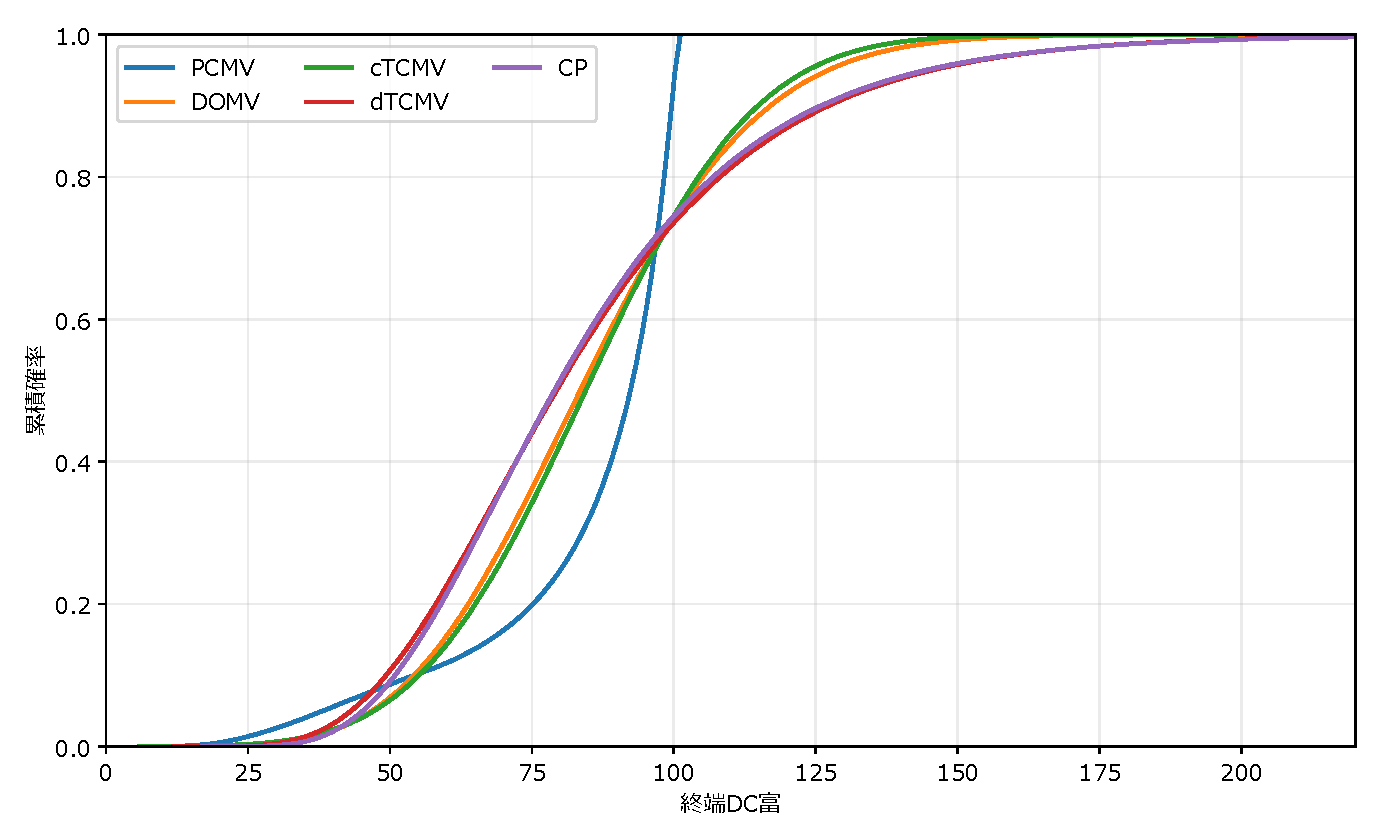
\includegraphics[width=.94\textwidth]{terminal_cdf_v9.pdf}
\caption{共通期待終価へ再較正した5戦略の終価CDF．独立100万経路の経験分布を分位点で要約した曲線．旧格子の分布ではない．}\label{fig:recalibrated_cdf}
\end{figure}

\subsection{平均配分と状態別方策を合わせて読む}
図\ref{fig:recalibrated_glide}の平均配分は，各方策が生成する残高分布に依存する．したがって，曲線間の差は同じ状態における方策差とは限らない．図\ref{fig:heatc}と図\ref{fig:heatd}は，時点と残高を固定した配分表を示す．固定残高範囲全体を描いており，到達確率の包絡で切り取った図ではない．

cTCMVとdTCMVの違いを単なる年齢別の曲線として捉えると，状態依存性を見落とす．dTCMVでは富依存係数によって現在の総年金富が目的へ入り，cTCMVでも残高制約と将来の制約拘束を通じて状態依存性が生じる．個別化という性質はdTCMVにだけ存在するわけではない．図の細かな帯は有限制御・状態近似の影響も受けるため，連続時間の自由境界そのものとは解釈しない．

\begin{figure}[htbp]\centering
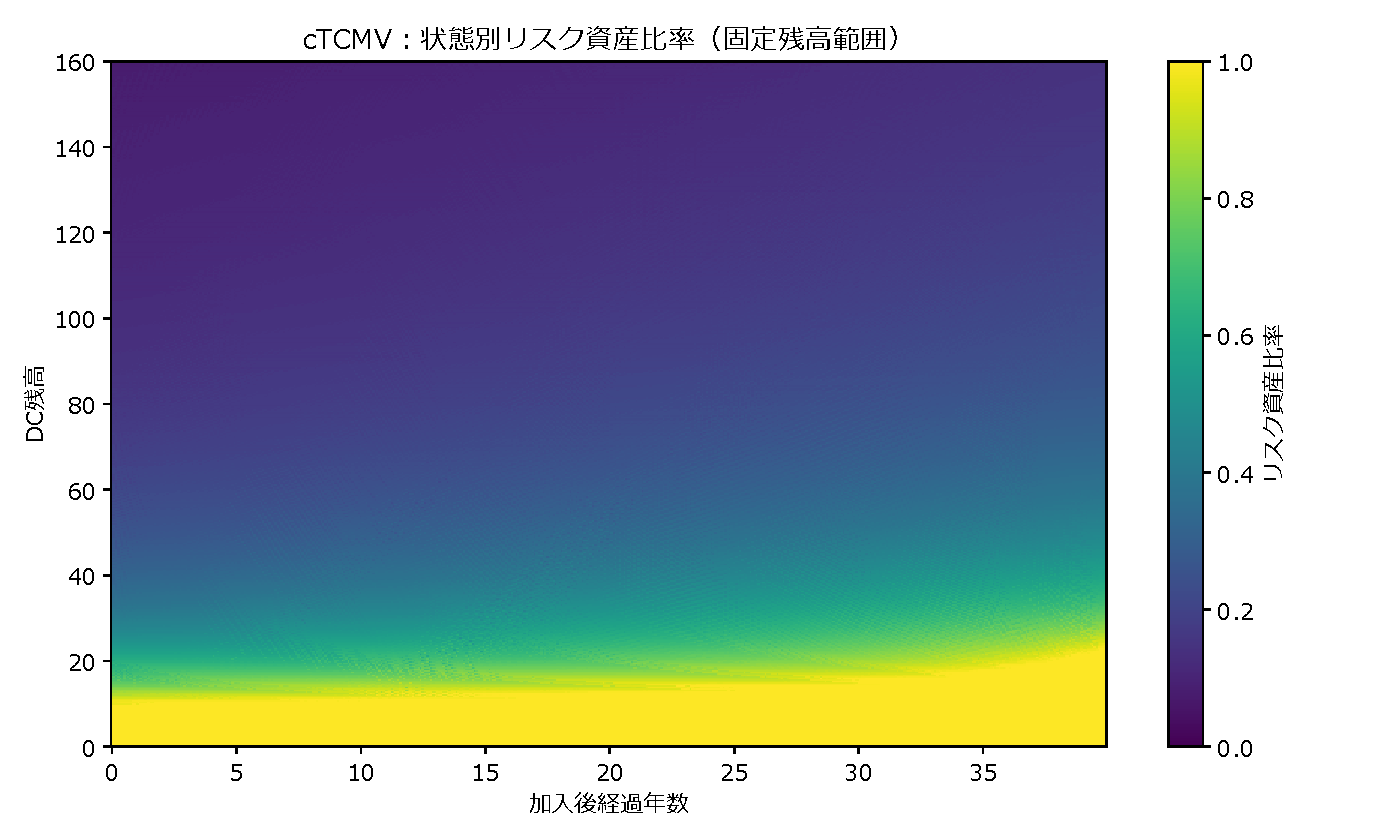
\includegraphics[width=.94\textwidth]{heatmap_cTCMV_v9.pdf}
\caption{新較正cTCMVのリスク資産比率．状態範囲は0より大きく160以下．各色は同じ時点・残高での方策を表す．}\label{fig:heatc}
\end{figure}

\begin{figure}[htbp]\centering
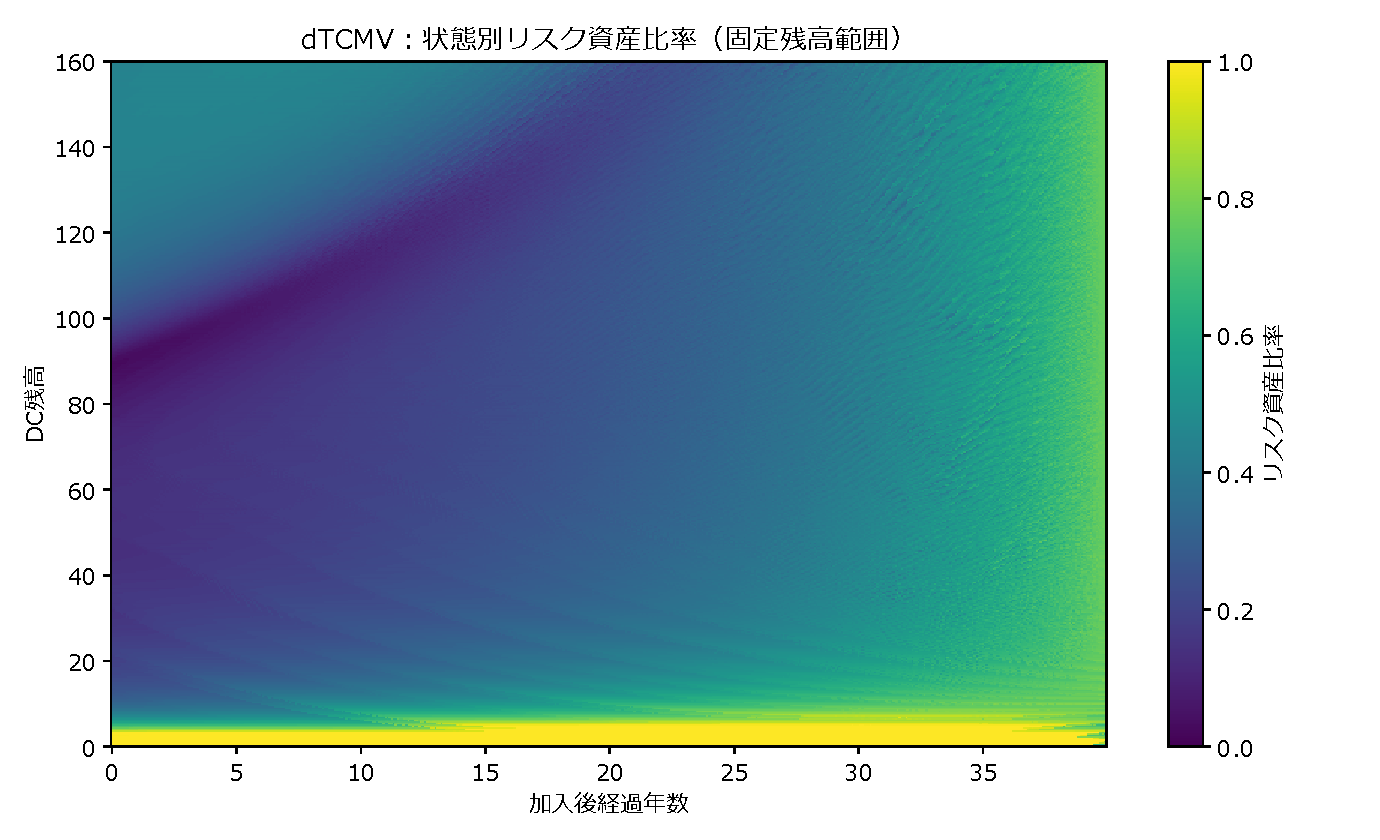
\includegraphics[width=.94\textwidth]{heatmap_dTCMV_v9.pdf}
\caption{新較正dTCMVのリスク資産比率．前図と同じ状態範囲・カラースケールを使用．}\label{fig:heatd}
\end{figure}
\subsection{裾指標の不確実性}
下位5\%平均には，100個の独立ブロックを用いる近似95\%区間を追加した（付録\ref{app:outcomes}）．図\ref{fig:tailci}は点推定の違いを標本誤差と併せて示す．これは各指標の周辺区間であり，全戦略の順位を同時に保証する検定ではない．また，標本誤差が小さくても，モデル係数や状態近似の系統誤差が小さいことにはならない．

\begin{figure}[htbp]\centering
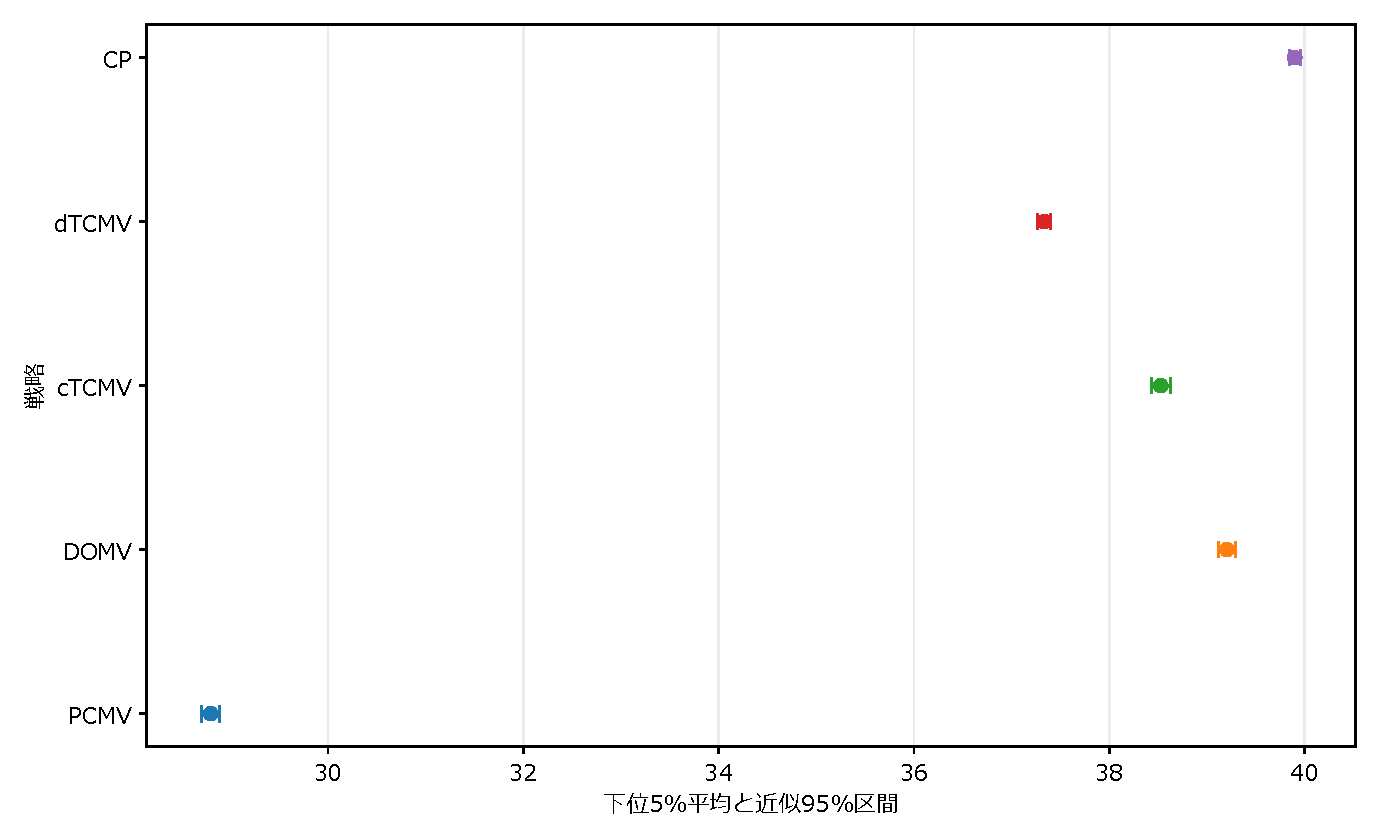
\includegraphics[width=.94\textwidth]{tail_intervals_v9.pdf}
\caption{下位5\%平均とブロックに基づく近似95\%区間．入力は新較正方策の100万経路．多重比較補正は行っていない．}\label{fig:tailci}
\end{figure}
\FloatBarrier
\section{新較正方策の状態別退職成果と年金実務}
\label{sec:rolling}
\subsection{同じ残高からの継続方策比較}
初期時点で平均をそろえても，途中の同じ残高からの条件付き平均は一致しない．この差は，各運用原理を継続したときの便益と費用を説明する情報になる．本節は旧方策の数値を流用せず，第\ref{sec:equalmean}節の新較正方策を用いて追加計算した．

開始状態は20年・残高20，30年・残高45，35年・残高30とする．それぞれ説明用に固定した状態であり，新分布の特定分位点とは主張しない．各状態で20万経路を用い，同じ市場ショックを5戦略に与える．条件付き平均を再びそろえるための係数変更は行わない．PCMVは初期に定めたターゲットの継続方策を実行する．

Markov方策$j$の条件付き平均を$\mu_j(t,x)$，分散を$v_j(t,x)$とすると
\begin{equation}
\Var(W_T^j)=\E[v_j(t,X_t^j)]+\Var(\mu_j(t,X_t^j)).\label{eq:totalvar}
\end{equation}
これは全分散の公式であり，初期設計評価と途中評価を結ぶ既知の恒等式である．条件付き比較は，加入者が既に観測した現在状態から先の問題に答える．
\begin{table}[htbp]\centering\small
\caption{新較正方策の共通状態からの成果（各20万経路）}\label{tab:rolling}
\begin{tabular}{llrrrrr}\toprule 状態$(t,x)$ & 方策 & 平均 & SD & q05 & LCVaR$_{5\%}$ & q95\\\midrule
(20,20) & PCMV & 73.48 & 22.10 & 28.78 & 22.86 & 97.50 \\
 & DOMV & 66.02 & 16.33 & 39.75 & 33.71 & 93.56 \\
 & cTCMV & 67.98 & 18.01 & 38.46 & 31.38 & 97.84 \\
 & dTCMV & 69.78 & 25.15 & 36.93 & 32.11 & 116.49 \\
 & CP & 67.75 & 21.55 & 39.44 & 35.18 & 107.71 \\
\midrule
(30,45) & PCMV & 75.91 & 17.15 & 38.74 & 31.36 & 95.04 \\
 & DOMV & 70.21 & 10.33 & 53.23 & 48.97 & 87.28 \\
 & cTCMV & 72.14 & 13.02 & 50.71 & 45.28 & 93.60 \\
 & dTCMV & 77.88 & 24.61 & 44.60 & 39.46 & 123.50 \\
 & CP & 74.85 & 18.77 & 48.54 & 44.06 & 109.14 \\
\midrule
(35,30) & PCMV & 44.82 & 15.77 & 22.81 & 19.70 & 74.15 \\
 & DOMV & 40.72 & 6.45 & 30.16 & 27.45 & 51.35 \\
 & cTCMV & 42.07 & 9.15 & 27.00 & 23.27 & 57.16 \\
 & dTCMV & 42.53 & 10.91 & 27.13 & 24.46 & 62.33 \\
 & CP & 40.96 & 7.26 & 30.21 & 28.12 & 53.88 \\
\bottomrule\end{tabular}\end{table}

\begin{figure}[htbp]\centering
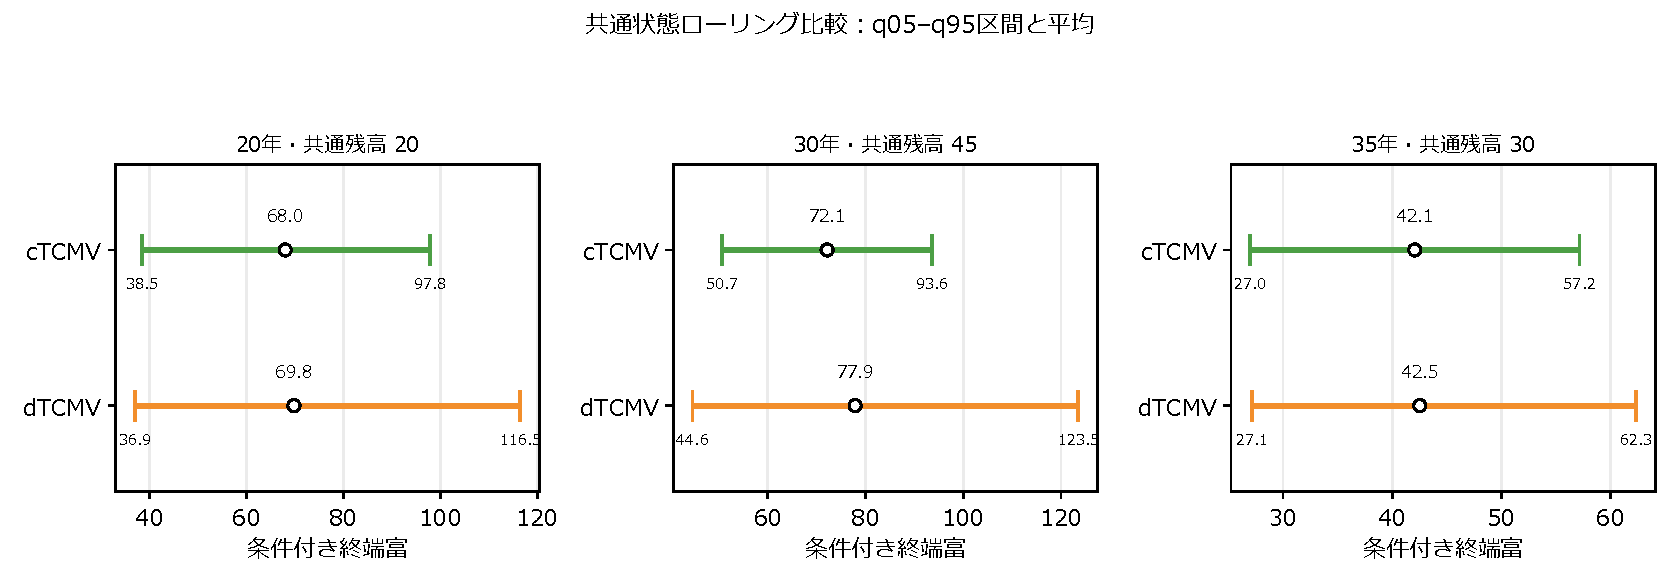
\includegraphics[width=1.0\textwidth]{rolling_v9.pdf}
\caption{新較正cTCMV・dTCMVの共通状態比較．横線はq05からq95，白丸は平均．v5の三面図の形式を踏襲し，入力を新方策へ更新した．}\label{fig:rolling-new}
\end{figure}

\subsection{状態によって変わる便益と費用}
30年・残高45では，dTCMVの平均はcTCMVより約5.74高い一方，下位5\%平均は約5.82低い．平均の差に対する共通乱数の近似95\%区間は$[5.68,5.79]$である．期待成果と下方保護の交換が明瞭に現れる．

一方，35年・残高30では，dTCMVの平均は約0.46高く，下位5\%平均も約1.19高い点推定となった．20年・残高20では，下位5\%点と下位5\%平均の差の向きも同一ではない．したがって，「dTCMVはどの状態でも下位裾を悪化させる」という一般化は，新較正の条件付き評価からは支持されない．この三状態は網羅的検査ではなく，状態依存性を示す例である．

\subsection{所得と不足額への翻訳}
年額拠出$C$と確定年金現価係数$\mathfrak a_T$を用いる説明用換算を
\begin{equation}
I_T=CW_T/\mathfrak a_T\label{eq:income}
\end{equation}
とする．$C=30$万円，$\mathfrak a_T=20$なら富1は年額1.5万円である．30年・残高45でdTCMVへ変更する例では，期待年額所得の差は約8.60万円，下位5\%平均所得の差は約$-8.74$万円となる．35年・残高30では，それぞれ約0.69万円，約1.79万円の増加である．これは実際の年金商品の価格を計算したものではない．

不足確率$\Pr(W_T<60)$と期待不足額$\E[(60-W_T)_+]$も区別する．30年・残高45ではcTCMVが約17.50\%・1.23，dTCMVが約24.42\%・2.33である．35年・残高30ではcTCMVが約97.52\%・18.02，dTCMVが約93.18\%・17.97であり，高い不足確率は方策変更だけで十分な目標達成が難しい状態であることを示す．拠出額，退職時期，目標の再検討を投資配分とは別の判断として説明する必要がある．
\subsection{採用判断のための検証手順}
\label{sec:practice}
制度運営者は，特定の解概念を商品名へ直結させる前に，次の条件を運用仕様として定める．
\begin{enumerate}[leftmargin=2em,itemsep=3pt]
\item 退職所得目標，拠出の確実性，背景富の扱いおよび分散・不足額・下位裾の許容水準を決める．
\item 初期計画を維持するか，逐次見直すか，将来の自己との均衡を使うかを選ぶ．
\item PCMVのターゲットまたは選好係数をそろえ，直接制約方策とクリップを同じ評価モデルで比較する．
\item 解析特殊例，一段階残差，独立分布評価，残高・制御・時間格子，境界および共通平均較正を監査する．
\item 同じ加入者状態での期待所得と下方所得を説明し，手数料，売買可能商品，更新頻度を加えた結果で採用を判断する．
\end{enumerate}
例えば，年額所得のLCVaR差を許容幅$\varepsilon_I$以内とするなら，終端富の許容幅は$\varepsilon_W=\mathfrak a_T\varepsilon_I/C$となる．実務上の許容誤差を年金所得単位から決め，数値精度の採否へ戻す点に意味がある．閾値は加入者属性と制度目的に応じて定め，本稿の例示値を一律に採用しない．

cTCMVは定数係数のため説明しやすい候補，DOMVは残存期間問題を見直す候補，dTCMVは背景富を反映する候補である．しかし，これだけで標準デフォルト，定期見直し，個別化助言への最適な割当てが実証されたわけではない．PCMVにも拠出・残高を通じた状態依存性があり，個別化はdTCMVに固有ではない．複数方策を切り替える運用は別の方策となるため，切替後の分布を改めて評価する．

\FloatBarrier
\section{限界と今後の研究}
\label{sec:limits}
第\ref{sec:equalmean}節で，共通有限モデル内の再最適化と期待終価84.78への再較正を実施した．残る課題は，連続時間・連続制御への誤差をさらに定量化することである．有限制御集合での全数探索，DOMVターゲット値の誤差上界，標本点における連続制御監査はそれぞれ保証範囲が異なる．月次モデルの数値比較を，すべての許容連続時間方策に対する厳密な順位の証明と解釈しない．

第二に，係数が既知という仮定を緩め，期待超過収益，変動性，インフレ，手数料の誤推定を含める必要がある．本稿のパラメータは例示値であり，特定市場の最新推定値ではない．第三に，確率的給与・拠出停止・死亡・複数資産を扱い，蓄積期と退職後取崩しを同じ所得目標で接続する．これらは所得状態や年金化価格などを追加する別の制御問題となる．

理論面では，制約付き均衡の大域存在・一意性，DOMVの共同可測なフィードバック選択と閉ループの適切性，離散均衡の連続時間収束が残る．正の歪度選好を持つMVSは，これらの基本的検証の後に位置づける（付録\ref{app:mvs-extended}）．

\FloatBarrier
\section{結論}
制約を満たすこと，制約付き最適化を再現すること，退職成果を正確に評価することは，三つの異なる要件である．本稿は四つの動的平均--分散解概念を整理し，固定ターゲット損失の残差表示，補間による追加分散，無制約係数のモーメント検証および独立分布評価を一つの検証手順へまとめた．

共通期待終価への再最適化では，分散と下位裾が異なる評価軸であることを再確認した．有限モデルの最適性と独立評価の数値精度を分け，較正係数・方策・検証データを公開する．参照計算では，内部モーメント一致があっても定率運用の分散精度に問題が残り，保存方策の共通平均較正も独立評価で維持されなかった．旧クリップ監査は同係数または固定ターゲットの比較であり，新較正下の同平均クリップ比較は残課題である．新較正方策による同じ途中残高からの評価では，期待所得と下方成果の交換が状態により変わることを確認した．この結果は加入者に説明する具体的な材料となる．年金実務にとって重要なのは，複雑な方策を採用すること自体ではなく，採用する方策と説明する退職成果の双方について，独立に確認できる根拠を持つことである．


\clearpage\appendix
\FloatBarrier
\section{背景富，尺度変更と時間非整合性の補足}
\label{app:background}
\subsection{拠出価値の変換と投資制約}
一定の年額拠出$c$，一定金利$r\ne0$の下では，背景富は
\begin{equation}
H_t=\frac{c}{r}\{1-e^{-r(T-t)}\}+D_Te^{-r(T-t)}.
\end{equation}
$r=0$では連続極限$H_t=c(T-t)+D_T$を用いる．$\dd H_t=(rH_t-c)\dd t$を状態方程式へ加えると拠出項が消え，$Y=X+H$の動学を得る．しかし，許容投資額は$0\leq\pi\leq Y-H$であり，$0\leq\pi\leq Y$へ置き換わらない．変数変換によって拠出を消すことと，将来拠出の証券化を認めることは別である．

時点$t$でDC残高が20，将来拠出価値が15であれば，総年金富は35である．無制約式が総年金富の80\%をリスク資産へ配分すると投資額は28となり，口座残高20を超える．事後クリップは20へ制限する．一方，直接制約問題は将来も同様の上限に直面する可能性を考慮して現在の投資を選ぶため，常に20を選ぶとは限らない．この数値例は制約の意味を説明する仮例であり，較正結果ではない．

\subsection{確定DB給付の平行移動と選好}
任意の定数$D$について
\begin{equation}
\E[X_T+D]-\frac\gamma2\Var(X_T+D)
=\E[X_T]-\frac\gamma2\Var(X_T)+D.
\end{equation}
取引集合が変わらず$\gamma$も固定なら，加算定数は最適化に影響しない．この議論は定数係数のPCMV，DOMV，cTCMVへ適用できる．固定ターゲット損失では$(X_T+D-m)^2=(X_T-(m-D))^2$であるため，同じDC目標を比較するには総富ターゲットを平行移動する．

dTCMVでは$\Gamma=\rho/(x+H_t)$自体が$D$に依存する．このため，同じDC残高でも背景給付が大きいほどモデル上の分散回避係数が低くなる．これは富依存選好を採用したことの帰結であり，DBの保有がすべての加入者の実際の選好を同じ方向へ変えるという命題ではない．確定額$D$の扱いと，死亡・金利によって変動する年金現価の扱いも区別する必要がある．

\subsection{単位変更に対する整合性}
金額を$k>0$倍すると，$\widetilde W=kW$に対して
\begin{equation}
\E[\widetilde W]-\frac{\widetilde\gamma}{2}\Var(\widetilde W)
=k\left\{\E[W]-\frac{k\widetilde\gamma}{2}\Var(W)\right\}.
\end{equation}
したがって$\widetilde\gamma=\gamma/k$なら選好を保つ．富依存型では$\widetilde\Gamma=\rho/(k(x+H))=\Gamma/k$となり，同じ$\rho$で尺度整合性を持つ．ただし，残高だけを増やし，将来拠出を増やさない比較は単なる単位変更ではない．この場合は実際の経済状態が変わっている．

成果を年額所得へ換算する場合も，係数と単位の対応を保つ．本稿の残高単位が年額拠出$C$に等しく，確定年金現価係数が$a$なら，年額所得は$I=CW/a$となる．係数の数値を別の金額単位へそのまま移植すると，意図しないリスク選好を与えることになる．

\subsection{全分散の公式と再計画}
初期時点での目的を，途中情報$\mathcal F_t$で分解すると
\begin{align}
\E[W_T]-\frac\gamma2\Var(W_T)
&=\E\left[\E[W_T\mid\mathcal F_t]-\frac\gamma2\Var(W_T\mid\mathcal F_t)\right]\notag\\
&\quad-\frac\gamma2\Var\left(\E[W_T\mid\mathcal F_t]\right).
\label{eq:time-inconsistency-explained}
\end{align}
途中時点で状態を観測した自己は，実現していない他の状態の条件付き平均とのばらつきを，同じ形では最適化しない．このため，初期に選んだ継続計画と，実現状態から再計画した方策が一致するとは限らない．式\eqref{eq:time-inconsistency-explained}は既知の条件付き期待値・分散の恒等式であり，本稿独自の新定理ではない．

DOMVはこの再計画を意思決定規則に含める．TCMVは将来の自己も意思決定することを予見した均衡として定式化する．PCMVは初期計画へコミットする．どの概念を採用するかは，数理的な都合だけでなく，制度がどのような運用契約・見直し規則を実装するかという仕様に関わる．

\subsection{三層構造を設計仮説として用いる条件}
標準運用，定期的な運用見直し，個別化助言という三つの実務機能を分けることは有用である．ただし，それぞれをcTCMV，DOMV，dTCMVへ機械的に割り当てることは本稿の数値結果からは導かれない．標準運用では運用費用と説明可能性，見直しでは再設定時の目的と継続責任，個別化では入力情報の品質と適合性が追加の判断要素となる．

具体的には，同じ残高・拠出計画から，単純な定率運用，クリップ近似，直接制約方策を比較する．期待所得だけでなく不足額を示し，変更後の目標と係数を記録する．当初のPCMV計画からの変更は，元計画の実装誤差ではなく，運用原理の変更である場合がある．この区別を明示して初めて，三層という整理を加入者への説明に利用できる．

\FloatBarrier
\section{埋め込み問題と均衡方程式の導出補足}
\label{app:derivations}
\subsection{二次損失とスカラー化目的の恒等式}
方策$\pi$の終価平均を$a_\pi$，分散を$v_\pi$とする．二次損失は
\begin{equation}
\E[(W_T-m)^2]=v_\pi+(a_\pi-m)^2.
\end{equation}
右辺を平方完成すると
\begin{equation}
m-\frac1{2\gamma}-\frac\gamma2\E[(W_T-m)^2]
=a_\pi-\frac\gamma2v_\pi-\frac\gamma2(m-a_\pi-1/\gamma)^2.
\end{equation}
任意の固定方策で右辺は$m=a_\pi+1/\gamma$において最大となる．方策と$m$に関する上限の順序を交換し，固定$m$について二次損失を最小化すれば本文の外側最大化が得られる．ここで使うのは積集合上の上限の交換であり，最適制御の存在や一意性を自動的に証明する操作ではない．

固定ターゲット最適方策$\pi_m$が平均$d_m$を達成するとする．同じ平均$d_m$の任意の許容方策$\nu$について
\begin{equation}
\Var(W_T^{\pi_m})+(d_m-m)^2
\leq\Var(W_T^\nu)+(d_m-m)^2
\end{equation}
だから最小分散性が従う．この論証では達成平均を事後的に指定しており，任意の目標$d$に対応する$m$の存在は別問題である．離散制御ではパラメータの微小変化で選択制御が切り替わり，平均写像が滑らかでない場合もある．

\subsection{固定点条件の限界}
スカラー化目的の最適な組$(\pi^*,m^*)$では，必要条件$m^*=a_{\pi^*}+1/\gamma$を満たす．しかし，この等式を満たす候補が複数存在するとき，すべてが大域的に最適とは限らない．各候補の埋め込み目的値を比較する必要がある．数値的に固定点反復が停止したという事実も，探索範囲外により良い候補が存在しないことを保証しない．

DOMVでは各状態の外側最適化で選んだターゲットを，次の時点までしか固定しない．その状態で計画した終価分布と，後続時点でも新しいターゲットを選び直して実現する分布は異なり得る．本稿の成果評価は後者を対象とし，PCMVターゲット群の計画平均をそのままDOMVの実現平均として使わない．

\subsection{局所均衡のモーメント展開}
将来方策を$\hat\pi$に固定し，現在の自己の係数を$\Gamma_0=\Gamma(t,x)$と書く．短時間$h$だけ別の許容制御を用いた後の一次・二次モーメントは
\begin{align}
F_h&=F+h(F_t+\mathcal L^\nu F)+o(h),\\
G_h&=G+h(G_t+\mathcal L^\nu G)+o(h).
\end{align}
目的$F_h-\Gamma_0(G_h-F_h^2)/2$を展開すると
\begin{equation}
J_h-J_0=h\left[(1+\Gamma_0F)(F_t+\mathcal L^\nu F)
-\frac{\Gamma_0}{2}(G_t+\mathcal L^\nu G)\right]+o(h).
\end{equation}
現在の自己を固定するため，この展開で$\Gamma_x$を生成作用素に入れない．将来の各状態では将来の自己の係数を用いるが，それは継続方策$\hat\pi$に含まれている．この二つの役割を分けることが富依存均衡の定式化で重要である．

制御に依存する部分は$\beta\pi A_F+\sigma^2\pi^2B_F/2$となる．$B_F<0$なら凹二次式であり，停留点の区間射影を取る．$B_F>0$なら最大値は端点にあり，$B_F=0$なら線形式の符号によって端点または全区間の同点となる．局所的な曲率条件を確認せず射影式だけを適用してはならない．

\subsection{自由境界という表現の範囲}
凹性が成り立つ領域で，射影前の投資額を$\phi(t,x)$とすると，下限制約は$\phi\leq0$，内点は$0<\phi<x$，上限制約は$\phi\geq x$に対応する．しかし$\phi$は制約付き値関数または均衡モーメントの微分に依存する未知量である．無制約問題の既知の$\phi^0$をクリップして得る境界とは一般に異なる．

この分類は切替集合の特徴づけであり，境界が常に一本の滑らかな曲線であることや，時間・残高に対して単調であることを意味しない．離散方策のヒートマップに段差や帯が見えても，それを直ちに連続時間の自由境界と同一視しない．特にゼロ残高では両端点が一致しており，制御の経済的な選択肢は一つだけである．

\subsection{無制約dTCMVの係数を再現する二つの表示}
本文の$a,b$を用い，残存期間を$\tau=T-t$とする．終端条件は$a(0)=b(0)=1$であり，
\begin{align}
\frac{\dd a}{\dd\tau}&=(r+\beta\theta)a,\qquad
\frac{\dd b}{\dd\tau}=(2r+2\beta\theta+\sigma^2\theta^2)b,\\
\theta&=\frac{\beta}{\rho\sigma^2}(a/b+\rho a^2/b-\rho).
\end{align}
別表示として$u=a/b$，$v=a^2/b$を用いれば
\begin{align}
\frac{\dd u}{\dd\tau}&=-(r+\beta\theta+\sigma^2\theta^2)u,
&u(0)&=1,\\
\frac{\dd v}{\dd\tau}&=-\sigma^2\theta^2v,
&v(0)&=1.
\end{align}
この二つのODEを独立に実装して比較すると，符号・指数の取り違えを検査できる．$\tau=0$では$\theta=\beta/(\rho\sigma^2)$であるが，これは退職直前の係数の極限であり，終端時点で新たな取引を行う指示ではない．

\FloatBarrier
\section{有限モデルのアルゴリズムと検証の詳細}
\label{app:algorithm}
\subsection{一つの遷移核を定める手順}
時点$n$，残高$x_i$，投資額$p$，正規化GH節点$\xi_k$から，
\begin{equation}
y_k=x_i+(rx_i+c_n+\beta p)\Delta t+\sigma p\sqrt{\Delta t}\xi_k
\end{equation}
を求める．有限モデルでは$[0,L]$へ境界処理した後，隣接格子へ非負の線形重みで配分する．この重みとGH重みの積が遷移確率となる．その総和は1であり，同じ配分を後退期待値と前進確率に用いる．上端で線形外挿する後退計算と，上端へ質量を集約する前進計算を混在させれば，同一核ではなくなる．

投資額を$P_{n,i}$として保存し，格子外の残高では投資額を補間する．比率$P_{n,i}/x_i$を補間する方法は一般に同じではない．特に$x=0$では投資額は0に定まるが比率の値は便宜的であり，その値を使った初期比率平均は人工的な低下を生み得る．初期残高は1/12から直接最初の遷移を行う．

\subsection{後退計算の三つの型}
固定ターゲットPCMVは，終端損失$(x_i-m)^2$から後退し，各状態で次期損失の期待値を最小化する．選択した投資額と継続平均を保存する．cTCMV・dTCMVは終端一次・二次モーメント$x_i,x_i^2$から後退し，次期モーメント$f(p),q(p)$を用いて
\begin{equation}
f(p)-\frac{\Gamma_{n,i}}2\{q(p)-f(p)^2\}
\end{equation}
を有限候補から最大化する．dTCMVの背景富は月次の割引再帰と整合させる．

DOMVはターゲットごとのPCMV損失群$V_{n,i}^{m}$と現在投資額を準備し，$m-\gamma_DV_{n,i}^{m}/2$を最大にするターゲットを各状態で選ぶ．定数$-1/(2\gamma_D)$は選択に影響しない．選んだ現在投資額を接続して実行方策を構成し，その方策を改めて評価する．ターゲット群の値を保存する段階と，実行分布を計算する段階は明確に分かれる．

\subsection{ターゲット範囲と離散化誤差の証明}
有限モデルの終価が$0\leq W\leq L$であるとする．スカラー化最適方策の平均$m_*$を用いると，埋め込みターゲットは$z_*=m_*+1/\gamma$であり，$z_*\in[1/\gamma,L+1/\gamma]$で足りる．本計算の$L=600$，$\gamma\geq0.02$では上端650を含む探索範囲を用いる．

最大間隔$\delta$のターゲット格子が$z_*$を挟むと，最近点$z_g$は$|z_g-z_*|\leq\delta/2$を満たす．元の最適方策を$z_g$で評価したときの目的低下は平方完成の恒等式により$\gamma(z_g-z_*)^2/2$である．$z_g$で内側方策を再最適化すればこの値より悪くならないため，
\begin{equation}
0\leq J^*-J^*_{\rm target\ grid}\leq\frac{\gamma\delta^2}{8}.
\end{equation}
この証明は有限モデル内の局所PCMV埋め込み値についてのものである．DOMVが後続時点でターゲットを切り替えることによる最終成果の誤差や，境界$L$そのものの近似誤差を含まない．

\subsection{全補間境界による一段階制御監査}
固定されたGH節点に対して$y_k(p)$は$p$のアフィン関数である．$y_k(p)$が富格子点を通過する全投資額を求め，許容区間の両端と合わせて並べる．各隣接区間では，補間された次期一次・二次モーメントの期待値はそれぞれ$p$のアフィン関数となる．このときMV目的の二階微分は$\Gamma(f'(p))^2\geq0$であり，最大値は区間端点にある．

従って，すべての通過点と端点を評価すれば，固定された継続モーメントに対する一段階の連続投資額最大化を実行できる．これは滑らかな凹関数を仮定した局所放物線補間とは異なる．ただし，計算量は節点数と格子数に依存する．本稿の主計算は有限比率集合の全数探索であり，通過点探索は指定時点・残高での補助監査である．この監査だけから，全状態で誤差が同じ上限以下だとは言わない．

\subsection{Bellman残差と方策損失の望遠和}
同じ有限核での最適固定ターゲット損失を$V_n$とし，ある方策$a_n$に対する残差を
\begin{equation}
r_n(x)=K_n^{a_n}V_{n+1}(x)-V_n(x)\geq0
\end{equation}
と定める．方策を実行した状態列について条件付き期待値を取れば，
\begin{equation}
\E[r_n(X_n)]=\E[V_{n+1}(X_{n+1})]-\E[V_n(X_n)].
\end{equation}
時点について足すと中間項が消え，終端損失の差が残差の到達確率加重和になる．よって，到達しない状態で大きな局所差があっても，その初期状態からの損失は小さい場合がある．逆に，小さな局所差が頻繁に到達する状態に集中すると累積損失が無視できない場合がある．

この恒等式を使うには，基準値関数，評価方策，初期状態，境界処理が同じでなければならない．異なるモデルや異なるターゲットの残差を混ぜて，純粋なクリップ誤差を測ったとは解釈できない．

\subsection{追加分散と時間刻みの関係}
状態配分の一段階追加分散は最大$h_x^2/4$である．これは局所的な上界であり，単純に$Nh_x^2/4$を最終誤差の厳密上界として使うには，遷移と方策の安定性に関する追加評価が必要である．ただし，時間刻みだけを小さくして配分回数を増やすと，状態近似の影響が自動的には減らないことを示唆する．

このため，時間刻み，状態刻み，制御候補，GH次数を個別に変えた診断に加え，それらの共同精緻化を検討する．本稿の主結果は月次モデルであり，連続時間への収束率を与えるものではない．正規Eulerの負残高を0へ切り上げる処理と，連続時間の非負性も同じ事実ではない．標本で負残高が観測されないことは，その処理の影響が標本内で見られなかったことを表す．

\subsection{定率方策のモーメント再帰}
定率$p=\theta X$では，Euler遷移は$X_{n+1}=A_nX_n+c\Delta t$，
\begin{equation}
A_n=1+(r+\beta\theta)\Delta t+\sigma\theta\sqrt{\Delta t}Z_n
\end{equation}
と書ける．$a=1+(r+\beta\theta)\Delta t$，$b=a^2+\sigma^2\theta^2\Delta t$とすると，配分前の平均$m_n$と二次モーメント$q_n$は
\begin{align}
m_{n+1}&=a m_n+c\Delta t,\\
q_{n+1}&=b q_n+2ac\Delta t\,m_n+c^2\Delta t^2.
\end{align}
初期条件は$m_0=x_0,q_0=x_0^2$である．この再帰には富格子が不要であり，数値評価の独立基準に使える．負残高切上げを組み込んだ過程では厳密には別の再帰になるため，解析式の対象を配分・切上げ前のEulerモデルと明示する．本設定での独立標本では負残高は観測されていない．

\FloatBarrier
\section{条件付き評価と退職所得指標の補足}
\label{app:outcomes}
\subsection{共通状態と自己の代表状態}
戦略$j$の分位状態$q_p(X_t^j)$から評価すると，その戦略を継続した典型的な加入者状態を説明できる．しかし$j$と$k$で分位状態の残高が異なるため，その終価差は現在資産の差と将来方策の差の両方を含む．一方，同じ$(t,x)$から評価すれば，将来方策を変更する効果を比較できる．

本稿の追加計算では$(20,20),(30,45),(35,30)$という三つの共通状態を固定する．これらはv8分布の特定の分位点と主張するものではなく，中期・退職前・低残高の比較を読むための説明用状態である．状態を固定した後に各方策を新しい共通平均へ再較正してはいない．従って条件付き平均の差は，その状態から元の運用仕様を継続する効果である．

\subsection{全期待値と全分散の適用}
$m_j(t,x)=\E[W_T^j\mid X_t^j=x]$，$v_j(t,x)=\Var(W_T^j\mid X_t^j=x)$と置くと
\begin{align}
\E[W_T^j]&=\E[m_j(t,X_t^j)],\\
\Var(W_T^j)&=\E[v_j(t,X_t^j)]+\Var(m_j(t,X_t^j)).
\end{align}
第一の分散項は，実現した各状態から先に残る不確実性の平均である．第二は，異なる状態に到達したことで将来の条件付き平均が異なる程度である．これは同一モデル内のシナリオ分解であり，共通市場に直面する現実の加入者集団の横断的格差をそのまま測定したものではない．後者を分析するには，加入年齢，所得，掛金，市場ショックの共通性などの集団モデルが必要となる．

この分解は無条件分散を小さくするPCMVの設計評価と，途中状態からの継続成果評価を矛盾なく併置する．途中状態である方策の期待値が高くなったことは，初期時点の同平均効率性に反するものではない．比較する条件と問いが異なっているからである．

\subsection{不足確率と期待不足額}
目標残高$b$に対して
\begin{equation}
P_b=\Pr(W_T<b),\qquad S_b=\E[(b-W_T)_+]
\end{equation}
を区別する．$P_b>0$なら，不足時の平均不足額は$S_b/P_b$である．$P_b$が小さくても$S_b/P_b$が大きい場合があるため，成功確率だけで選択すると深い不足を見落とす．また，目標$b$の変更によって順位が変わり得るため，一つの閾値による結論をすべての退職目標へ一般化しない．

確定換算係数$k=C/a>0$なら，$I=kW$に対して
\begin{align}
\Pr(I<i_*)&=\Pr(W<i_*/k),\\
\E[(i_*-I)_+]&=k\E[(i_*/k-W)_+],\\
q_\alpha(I)&=kq_\alpha(W),\qquad
\mathrm{LCVaR}_\alpha(I)=k\mathrm{LCVaR}_\alpha(W).
\end{align}
この正の線形変換は分位順位を保つ．一方，年金価格が確率的である場合，$\E[CW/a_T]$を$C\E[W]/\E[a_T]$へ置き換えられず，残高順位が所得順位へそのまま移る保証もない．

\subsection{ブロックによる裾指標の誤差評価}
初期時点の独立評価は100ブロック，各1万経路から構成される．各ブロックの下位5\%点，上位5\%点，下位5\%平均を計算し，指標のブロック間標準偏差を$\sqrt{100}$で割って近似標準誤差を求めた．全100万経路の推定値を中心に，約1.984標準誤差の区間を示す．

これは非線形指標の有限ブロックによる近似であり，ブロック推定量の小標本バイアスは完全には除去しない．多重比較補正を行った全順位の信頼集合でもない．平均差の同等性検査に用いたBonferroni補正とは区別する．分位密度が小さい領域や，離散的な分布に対しては，この誤差評価の安定性も確認すべきである．

\subsection{加入者説明で示す順序}
第一に現在の残高と残存拠出，第二に将来方策と初期配分，第三に期待所得と下位成果，第四に目標不足を説明する．高い期待所得を提示するだけでは，どの程度のリスクを追加したかが分からない．逆に，低い分散だけでは必要所得の達成に十分かが分からない．

本稿の所得換算は，年額拠出30万円，現価係数20という仮定を使う説明例であり，税，費用，遺族給付，保証期間，死亡率を含む保険商品の価格ではない．実際の採用では，この換算係数を加入者・制度の条件に合わせる工程が必要になる．

\FloatBarrier
\section{平均--分散--三次中心モーメント拡張の位置づけ}
\label{app:mvs-extended}
\subsection{通称としてのMVSと目的の単位}
MVSという名称で
\begin{equation}
J=\E[W]-\frac\gamma2\Var(W)+\frac\eta3\E[(W-\E[W])^3]
\end{equation}
を扱う場合，追加項は無次元の標準化歪度ではない．原始モーメントを$m_1,m_2,m_3$とすると，三次中心モーメントは$m_3-3m_1m_2+2m_1^3$である．単位整合性から$\eta$は金額の逆二乗となる．金額を$k$倍すると$\eta$も$1/k^2$倍する必要がある．

同じ分散でも左右非対称性に選好を与えることは研究上意味があるが，三次項の係数を増やすことが下方保護を強めるとは限らない．大きな上方成果が三次項を支配し，下方成果を悪化させながら目的を上げる場合がある．高次モーメントは右裾打切りにも敏感である．

\subsection{解概念ごとの違い}
PCMV--MVSは初期の高次モーメント目的へコミットする問題であり，MVと同じ二次損失だけでは表現できない．DOMV--MVSでは残存期間の高次モーメント計画を更新するため，ターゲット・乗数探索と実行後成果の差がさらに重要になる．TCMV--MVSでは三次モーメントの継続関数を含む局所均衡条件が必要である．

\citet{MuTianYang2019}を踏まえたv5の整理は，無制約の特定設定におけるcTCMVSとcTCMVの一致，その共通解をクリップした方策の一致，直接制約下の一般的一致が未証明であることを区別していた．この区別は維持する．無制約の相殺構造を，状態依存制約が将来モーメントに入る問題へそのまま拡張してはならない．

dTCMV--MVSでは，$\Gamma=\rho/(x+H)$，$\eta=\xi/(x+H)^2$という尺度整合的な仕様が考えられる．ただし，$\xi$の選択を加入者の実証的選好と呼ぶには，別の較正根拠が必要である．MVへ戻す$\xi=0$の入れ子検査は実装検証として有用だが，正の$\xi$での大域解や数値安定性を保証しない．

\subsection{v5の探索結果を再利用する条件}
v5では粗い格子で複数ケースのq05が同じ点に載り，精緻化によって分離した事例を記録していた．これは経済的な分布一致を主張する結果ではなく，高次モーメント問題の格子感応度を示す診断である．同じ係数を保つ比較と，同じ平均へ再較正する比較も区別されていた．本稿ではこれらの問題意識を残し，旧MVS数表を新較正MVの結果へ混ぜない．

再利用には，第一に目的関数と係数単位，第二に非凹問題の探索範囲，第三に境界・状態・制御・時間刻みの感応度，第四に独立評価での裾指標を確認する必要がある．この順序が整うまでは，MVSを標準運用や個別化助言へ採用する追加層とはせず，研究拡張として位置づける．

\FloatBarrier
\section{実装・ガバナンスと拡張研究の設計}
\label{app:governance}
\subsection{モデル入力と運用判断の責任}
運用方策には，市場係数，拠出計画，残高，退職時点，給付の評価，選好係数が入力される．このうち市場係数の推定誤差と，選好係数の不確実性は別の問題である．共通平均較正は研究上の比較条件を作る操作であり，加入者の選好を推定した操作ではない．

運営主体が方策を採用する際は，目標と係数の設定者，更新頻度，例外時の取扱い，結果の監視方法を定める．モデルが計算した配分を説明するために，入力の意味を後から変更してはならない．特に将来拠出を固定した計算では，離職や拠出停止によって背景富の前提が変わることがある．

\subsection{クリップ近似の採用判定}
単純なクリップが有用かどうかは，計算の容易さだけでは決まらない．比較条件を固定し，到達確率の高い状態における配分差，期待値差，目標不足，裾差を測る．固定ターゲットのPCMVならBellman残差の加重和が目的損失の診断に使える．TCMVでは局所逸脱の条件と，実現分布の便益を分ける．

同じ係数の比較は，同じ選好仕様を近似できているかを問う．同じ期待値に再較正した比較は，同じ平均のためにどのリスク分布を選ぶかを問う．近似側の係数を変更すれば，純粋な方策近似とは別の比較になる．本稿の旧クリップ監査は前者の条件付き診断であり，新方策間の同平均比較へ流用しない．

\subsection{モデルを複雑化する順序}
費用を加える場合，定率費用と売買時費用は異なる．後者は方策の変更幅に依存し，現在保有比率等を状態へ加える必要がある．確率的所得を加える場合は，所得と市場の相関，拠出規則，所得の取引不可能性をモデルに含める．単に$H_t$へ平均所得を代入するだけでは同じ問題にならない．

死亡・長寿を加える場合は，積立期間の死亡給付，生存条件付き目標，退職後の給付期間を分ける．退職時の残高分布だけでは生涯所得の不足を評価できない．複数資産では許容集合と相関推定が増え，単一リスク資産の一段階端点探索をそのまま使えない．

従って，拡張は既存の数値検証を維持できる順序で進める．まず基本モデルの独立評価と再現性を固定し，次に一つの実務要素を加え，その要素が意思決定と成果をどの程度変えるかを比較する．多くの要素を同時に追加して変化の原因を不明確にすることを避ける．

\subsection{再現可能性と図表の管理}
図表は，入力方策の版，評価モデル，標本数，種，集計方法を追跡できる必要がある．グライドパスの平均は実現比率の平均であり，平均投資額を平均残高で割った比率とは異なる．方策ヒートマップは固定残高範囲を描くのか，到達分布で限定するのかを明示する．CDFを平滑化した密度と混同しない．

本稿の図は公開リポジトリの日本語作図スクリプトの横長比率，淡いグリッド，凡例と色系列を踏襲し，新較正方策のデータから再生成する．見た目の継続性は保つが，旧画像を新しい数値の証拠として再掲しない．再現パッケージには図のベクトルPDF，PNG，集計CSV，生成コードと入力版を含める．

\FloatBarrier
\section{再較正結果と追加検証の詳細表}
\label{app:numerical-tables}
\subsection{評価モデルと最適化モデルの対応}
本付録は本文の新較正結果を再現するための詳細を示す．「後退・前進」は同じ有限核，「決定論的評価」は別の細かい富格子，「独立評価」は残高を格子へ配分しない正規Eulerシミュレーションである．数値を比較するときは，どの列がどのモデルを表すかを確認する．

基準モデルと精緻化モデルは，状態刻みだけでなく制御候補と求積次数も変更している．この二つの結果の差を，状態刻み一つの純粋な因果効果とは解釈しない．評価だけを変更した感応度は，方策の再最適化を含む感応度と別に記録する．

\begin{table}[htbp]\centering\small
\caption{主計算・評価・追加分析の仕様}\label{tab:spec-detail}
\begin{tabular}{ll}\toprule
項目 & 設定 \\ \midrule
期間と意思決定 & 40年，480月次区間 \\
初期DC残高 & 1/12 \\
年額拠出と終端給付 & $c=1,\ D_T=0$ \\
市場係数 & $r=0.015,\ \beta=0.04,\ \sigma=0.18$ \\
基準有限モデル & 3001状態，65比率，GH5点 \\
精緻化有限モデル & 6001状態，129比率，GH7点 \\
共通富上端 & 600 \\
最終決定論的評価 & 富刻み0.025，GH31点 \\
初期状態の独立評価 & 100万経路，100ブロック \\
追加の途中状態評価 & 各20万経路，40ブロック \\
新較正の目標と許容差 & 84.78，絶対誤差0.01 \\
平均同等性の許容幅 & $\pm0.1$ \\
\bottomrule\end{tabular}\end{table}

\subsection{独立評価の終価分布と不足}
表\ref{tab:full-terminal}の中央値と上位点は，平均だけでは分からない分布形状を補足する．PCMVではターゲット近傍への圧縮が見られる一方，下位側に大きな不足が残る．この特徴は「平均--分散の効率性」と「下方保護」が異なることを示す．PCMVを否定する根拠でも，下位裾だけを唯一の目的とする根拠でもない．

\begin{table}[htbp]\centering\small
\caption{新較正方策の終価分布の補足（100万経路）}\label{tab:full-terminal}
\begin{tabular}{lrrrr}\toprule
方策 & 平均 & 中央値 & q05 & q95 \\ \midrule
PCMV & 84.772 & 92.350 & 38.194 & 100.225 \\
DOMV & 84.783 & 83.476 & 46.869 & 127.060 \\
cTCMV & 84.791 & 84.467 & 47.161 & 123.471 \\
dTCMV & 84.786 & 79.258 & 43.173 & 145.252 \\
CP & 84.785 & 78.930 & 45.227 & 144.186 \\
\bottomrule\end{tabular}\end{table}

\begin{table}[htbp]\centering\small
\caption{新較正方策の目標60に対する不足}\label{tab:full-shortfall}
\begin{tabular}{lrrr}\toprule
方策 & 不足確率 & 期待不足額 & 不足時平均不足 \\ \midrule
PCMV & 11.743\% & 2.3054 & 19.6326 \\
DOMV & 15.510\% & 1.6484 & 10.6277 \\
cTCMV & 14.330\% & 1.6004 & 11.1675 \\
dTCMV & 22.557\% & 2.4414 & 10.8234 \\
CP & 21.432\% & 2.0858 & 9.7322 \\
\bottomrule\end{tabular}\end{table}

不足時平均不足は，期待不足額を不足確率で割った量である．たとえばPCMVは不足確率が他の一部の戦略より低いが，不足時にはより深く不足する．DCの説明では，「成功する割合」と「失敗した場合の深さ」を並べることで，一つの数値による誤解を避ける．閾値60はこの設定の説明用目標であり，他の所得目標に対する順位は別途計算する．

\subsection{対応のある平均差の同等性}
同じショックを各方策へ与えると，差$D_b=W^{j}_b-W^{k}_b$を直接集計できる．平均差の標準誤差は，二つの平均SEを独立として合算するのではなく，差の標本標準偏差を標本数の平方根で割って求める．共通乱数による共分散を利用するためである．

表\ref{tab:paired-full}では10組を同時に扱うため，正規近似に基づくBonferroni補正を用いる．全区間が許容域内に入ることを平均同等性の条件とした．許容幅は比較設計上の選択であり，較正誤差の閾値とは異なる．年額拠出30万円・現価係数20なら富0.1は年額1500円に対応する．この換算は許容幅の大きさを理解する説明であり，その幅をすべての制度に推奨するものではない．

\begin{table}[htbp]\centering\small
\caption{全10組の平均差と近似同時95\%区間}\label{tab:paired-full}
\begin{tabular}{lrrr}\toprule
組（前者−後者） & 平均差 & 下限 & 上限 \\ \midrule
PCMV / DOMV & -0.01154 & -0.05033 & 0.02724 \\
PCMV / cTCMV & -0.01975 & -0.05293 & 0.01344 \\
PCMV / dTCMV & -0.01473 & -0.08244 & 0.05299 \\
PCMV / CP & -0.01386 & -0.07815 & 0.05043 \\
DOMV / cTCMV & -0.00820 & -0.02132 & 0.00492 \\
DOMV / dTCMV & -0.00318 & -0.06003 & 0.05366 \\
DOMV / CP & -0.00231 & -0.04460 & 0.03997 \\
cTCMV / dTCMV & 0.00502 & -0.04223 & 0.05227 \\
cTCMV / CP & 0.00589 & -0.03096 & 0.04274 \\
dTCMV / CP & 0.00087 & -0.02535 & 0.02709 \\
\bottomrule\end{tabular}\end{table}

\subsection{裾の周辺区間}
表\ref{tab:tails-full}は本文の下位裾図を補足する．ブロックを用いた近似標準誤差は，固定した方策に対する標本変動を評価する．方策を再推定したときの不確実性，市場パラメータの不確実性，離散化誤差をこの区間へ含めてはいない．また，同じ標本を新しい係数へ事後的に合わせる操作は行っていない．

\begin{table}[htbp]\centering\small
\caption{裾指標とブロックによる近似95\%周辺区間}\label{tab:tails-full}
\begin{tabular}{llrrrr}\toprule
方策 & 指標 & 推定値 & SE & 下限 & 上限 \\ \midrule
PCMV & q05 & 38.1937 & 0.0625 & 38.0696 & 38.3178 \\
PCMV & q95 & 100.2246 & 0.0036 & 100.2176 & 100.2317 \\
PCMV & LCVaR & 28.7985 & 0.0473 & 28.7047 & 28.8924 \\
DOMV & q05 & 46.8690 & 0.0383 & 46.7929 & 46.9450 \\
DOMV & q95 & 127.0602 & 0.0514 & 126.9582 & 127.1623 \\
DOMV & LCVaR & 39.2036 & 0.0440 & 39.1164 & 39.2908 \\
cTCMV & q05 & 47.1606 & 0.0395 & 47.0823 & 47.2389 \\
cTCMV & q95 & 123.4706 & 0.0508 & 123.3697 & 123.5715 \\
cTCMV & LCVaR & 38.5271 & 0.0499 & 38.4280 & 38.6262 \\
dTCMV & q05 & 43.1728 & 0.0272 & 43.1190 & 43.2267 \\
dTCMV & q95 & 145.2516 & 0.1012 & 145.0508 & 145.4523 \\
dTCMV & LCVaR & 37.3322 & 0.0325 & 37.2677 & 37.3968 \\
CP & q05 & 45.2269 & 0.0271 & 45.1731 & 45.2807 \\
CP & q95 & 144.1862 & 0.1127 & 143.9627 & 144.4097 \\
CP & LCVaR & 39.8995 & 0.0286 & 39.8427 & 39.9564 \\
\bottomrule\end{tabular}\end{table}

\subsection{内部モーメント一致と格子外の平均}
表\ref{tab:internal-full}の平均は，本文の較正用平均と完全には一致しない．この表は最適化に用いた有限核の中での値であり，本文は格子外評価を含めて係数を較正しているからである．一致すべき組は同じ表の後退・前進であって，異なるモデルの平均を無条件に同じと要求するわけではない．その一方，モデル間の差を無視してよいわけでもなく，別の精度診断で監視する．

\begin{table}[htbp]\centering\small
\caption{精緻化有限モデルの内部モーメント一致}\label{tab:internal-full}
\begin{tabular}{lrrrr}\toprule
方策 & 後退平均 & 前進平均 & 後退SD & 前進SD \\ \midrule
PCMV & 84.767259 & 84.767259 & 18.959384 & 18.959384 \\
cTCMV & 84.754123 & 84.754123 & 23.147057 & 23.147057 \\
dTCMV & 84.734491 & 84.734491 & 32.218096 & 32.218096 \\
\bottomrule\end{tabular}\end{table}

\begin{table}[htbp]\centering\small
\caption{新CP比率の解析SDと評価格子精緻化}\label{tab:cp-refine}
\begin{tabular}{lrrr}\toprule
評価格子刻み & 平均 & SD & 解析SDとの差 \\ \midrule
0.200 & 84.779991 & 32.024524 & 0.350601 \\
0.100 & 84.779993 & 31.745179 & 0.071256 \\
0.050 & 84.779993 & 31.692921 & 0.018998 \\
0.025 & 84.779993 & 31.678841 & 0.004918 \\
解析Euler & 84.780000 & 31.673923 & 0 \\
\bottomrule\end{tabular}\end{table}

\subsection{GH次数と境界変更}
表\ref{tab:gh-full}は新方策を固定し，評価のGH次数を変更した値である．特にcTCMV・dTCMVでは低い次数からの変化がPCMVより大きい．この結果は「同じ求積法を使った」だけでは精度が均一にならないことを示す．高次数間の差が小さいことも，時間・制御・境界を含む包括的収束の証明ではない．

\begin{table}[htbp]\centering\small
\caption{固定方策・富刻み0.025の求積次数感応度}\label{tab:gh-full}
\begin{tabular}{lrrr}\toprule
方策 & GH点数 & 平均 & SD \\ \midrule
PCMV & 9 & 84.781547 & 18.935217 \\
PCMV & 31 & 84.781390 & 18.935060 \\
PCMV & 61 & 84.781352 & 18.935025 \\
DOMV & 9 & 84.780147 & 24.409873 \\
DOMV & 31 & 84.781589 & 24.407741 \\
DOMV & 61 & 84.781956 & 24.408252 \\
cTCMV & 9 & 84.849236 & 23.217573 \\
cTCMV & 31 & 84.783547 & 23.144448 \\
cTCMV & 61 & 84.790144 & 23.153229 \\
dTCMV & 9 & 84.828467 & 32.397837 \\
dTCMV & 31 & 84.777185 & 32.299760 \\
dTCMV & 61 & 84.779489 & 32.306700 \\
CP & 9 & 84.779993 & 31.678841 \\
CP & 31 & 84.779993 & 31.678788 \\
CP & 61 & 84.779993 & 31.678767 \\
\bottomrule\end{tabular}\end{table}

\begin{table}[htbp]\centering\small
\caption{dTCMVの上端変更と再較正}\label{tab:cap-full}
\begin{tabular}{lrrr}\toprule
上端 & rho & 評価平均 & 評価SD \\ \midrule
600 & 1.61425781 & 84.777185 & 32.299760 \\
900（同係数） & 1.61425781 & 84.703351 & 32.242870 \\
900（再較正） & 1.61457031 & 84.778337 & 32.286962 \\
\bottomrule\end{tabular}\end{table}

上端変更は後退計算を変え，その影響が到達しやすい状態の方策へ伝わることがある．上端への到達頻度が小さいことだけで，方策の境界依存性を否定できない．再較正後の分散が近づくという観察は有用だが，すべての係数・均衡分枝に対する不変性を示すものではない．

\subsection{共通途中状態の行動と不足}
本文の条件付き分布表に，現在の投資比率と不足指標を加える．同じ状態で比較しても，現在比率が高い方策が必ず満期分散も高くなるわけではない．将来の残高変化とその後の方策が残存期間全体へ作用するためである．現在の行動と最終成果の両方を確認する必要がある．

\begin{table}[htbp]\centering\small
\caption{共通状態における現在の配分と将来不足}\label{tab:rolling-detail}
\begin{tabular}{llrrr}\toprule
$(t,x)$ & 方策 & 現在比率 & 不足確率 & 期待不足額 \\ \midrule
(20,20) & PCMV & 1.0000 & 25.00\% & 5.0187 \\
(20,20) & DOMV & 0.7969 & 36.36\% & 3.8990 \\
(20,20) & cTCMV & 0.7500 & 33.07\% & 3.8795 \\
(20,20) & dTCMV & 0.3906 & 39.82\% & 4.9294 \\
(20,20) & CP & 0.4689 & 41.03\% & 4.4908 \\
(30,45) & PCMV & 0.7188 & 17.09\% & 2.6410 \\
(30,45) & DOMV & 0.4062 & 16.12\% & 0.8748 \\
(30,45) & cTCMV & 0.4375 & 17.50\% & 1.2304 \\
(30,45) & dTCMV & 0.4531 & 24.42\% & 2.3308 \\
(30,45) & CP & 0.4689 & 21.89\% & 1.6411 \\
(35,30) & PCMV & 1.0000 & 80.56\% & 17.0725 \\
(35,30) & DOMV & 0.5234 & 99.86\% & 19.2780 \\
(35,30) & cTCMV & 0.7188 & 97.52\% & 18.0166 \\
(35,30) & dTCMV & 0.6172 & 93.18\% & 17.9692 \\
(35,30) & CP & 0.4689 & 98.81\% & 19.0917 \\
\bottomrule\end{tabular}\end{table}

\begin{table}[htbp]\centering\small
\caption{途中状態のdTCMV−cTCMV平均差}\label{tab:rolling-pairs}
\begin{tabular}{lrrrr}\toprule
$(t,x)$ & 差 & SE & 95\%下限 & 95\%上限 \\ \midrule
(20,20) & 1.80670 & 0.02503 & 1.75763 & 1.85576 \\
(30,45) & 5.73640 & 0.02854 & 5.68046 & 5.79233 \\
(35,30) & 0.45777 & 0.00609 & 0.44583 & 0.46972 \\
\bottomrule\end{tabular}\end{table}

これらの平均差の区間は各状態の周辺区間であり，三状態を同時に補正していない．状態間は別の乱数種を用い，各状態の内部では全戦略に共通乱数を与えた．負残高および600超過は追加標本内で観測されなかった．ただし，観測ゼロは到達確率ゼロの数学的証明ではない．

\subsection{追加分析の独立検査}
定率CPは途中状態からも解析モーメント再帰を利用できる．各状態の残存期間に対して再帰を適用し，独立MC平均が解析平均と標本誤差内で整合するかを確認する．また，q05以下の裾平均はq05を超えず，q05，中央値，q95の順序が保たれ，投資額は口座残高以下でなければならない．これらは比較の品質を支える検査であり，動的方策の最適性を証明するものではない．

\begin{table}[htbp]\centering\small
\caption{追加CP計算の解析平均との照合}\label{tab:rolling-cp-check}
\begin{tabular}{lrrr}\toprule
$(t,x)$ & 解析平均 & MC平均 & 差 / SE \\ \midrule
(20,20) & 67.75818 & 67.75262 & -0.115 \\
(30,45) & 74.91346 & 74.84902 & -1.536 \\
(35,30) & 40.94567 & 40.95548 & 0.604 \\
\bottomrule\end{tabular}\end{table}

\FloatBarrier
\section{退職目標を変えたときの不足分析}
\label{app:targets}
\subsection{一つの閾値に依存しない成果説明}
本文では目標60を用いたが，加入者が必要とする所得水準は一つではない．同じ方策・同じ終価標本を固定し，目標だけを変えると，不足の頻度と深さがどう変わるかを評価できる．ここでは20から130の範囲を描き，40，60，80，100を詳細表に示す．各閾値へ期待終価を再較正した結果ではない．

この分析の目的は，一つの指標の順位を普遍的な優劣に置き換えないことである．目標を高くすると不足確率が高まること自体は自然だが，その増加の仕方は分布形状に依存する．PCMVのターゲット近傍の圧縮，定率運用の右裾，均衡方策の状態依存性は，不足曲線の異なる領域へ現れる．

\begin{figure}[htbp]\centering
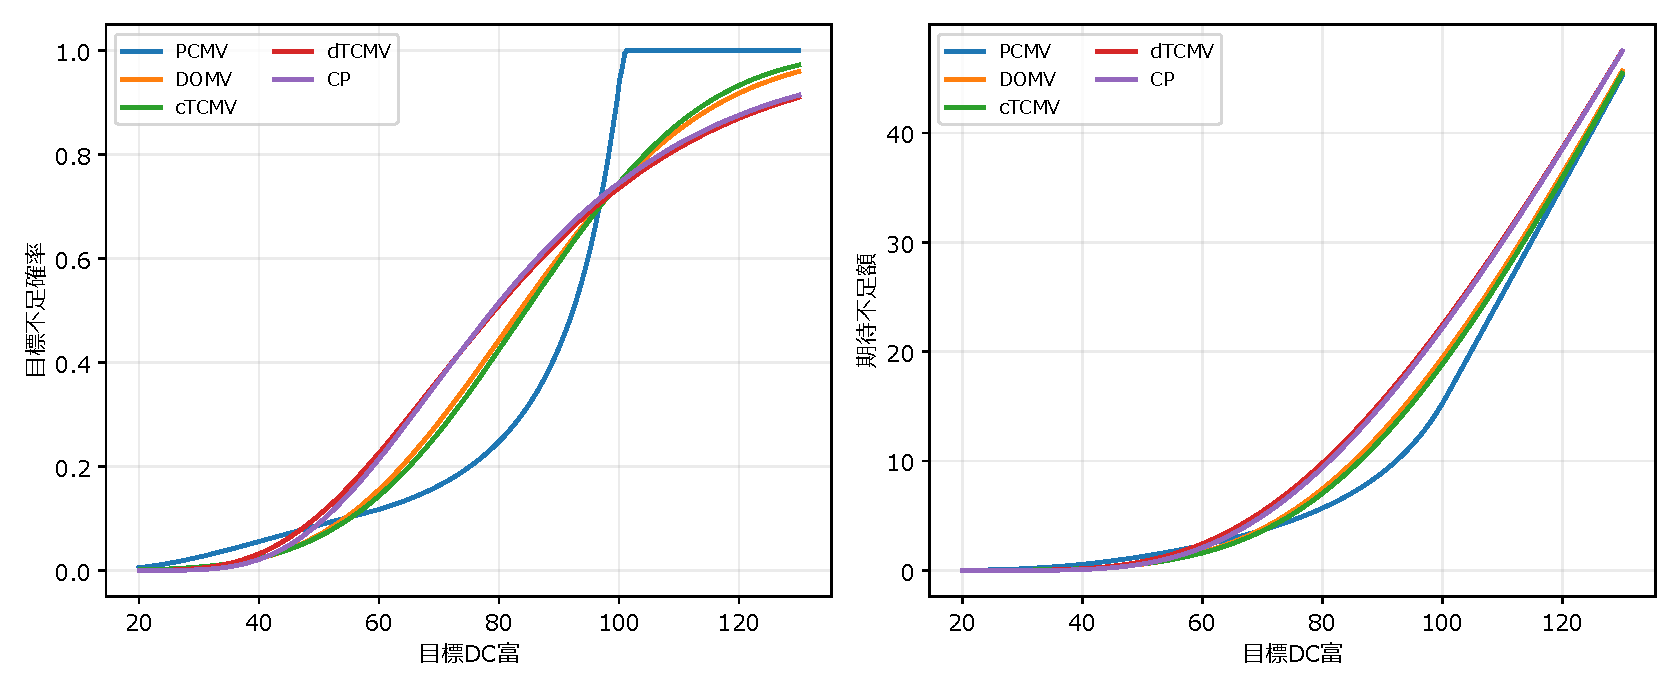
\includegraphics[width=\textwidth]{target_sensitivity_v9.pdf}
\caption{新較正5戦略の目標不足確率と期待不足額．同じ100万経路の標本で目標のみを変更．}\label{fig:targets}
\end{figure}

\subsection{確率と深さの関係}
非負終価$W$について，期待不足額は分布関数の積分として
\begin{equation}
S(b)=\E[(b-W)_+]=\int_0^b F_W(u)\dd u
\end{equation}
と表せる．したがって，連続点では$S'(b)=F_W(b)$であり，不足確率は不足額曲線の傾きを表す．ただし，ある一点で不足確率が小さいことだけでは，そこまで積分した期待不足額も小さいとは限らない．この関係が二つの指標を併記する理由である．

図\ref{fig:targets}の不足確率曲線が交差する場合，ある目標では有利な方策が，別の目標では不利となる．期待不足額でも同じ順位になるとは限らない．全目標での優位を論じるには，点の比較より強い分布の順序が必要であり，本稿は単一目標の比較から確率優越を主張しない．

\begin{table}[htbp]\centering\small
\caption{目標別の不足確率と期待不足額（新較正方策）}\label{tab:targets}
\begin{tabular}{rlrrrr}\toprule
目標 & 方策 & 不足確率 & 確率SE & 期待不足額 & 不足額SE\\\midrule
40 & PCMV & 0.0559 & 0.00023 & 0.5654 & 0.00283 \\
40 & DOMV & 0.0226 & 0.00015 & 0.1434 & 0.00124 \\
40 & cTCMV & 0.0238 & 0.00015 & 0.1770 & 0.00148 \\
40 & dTCMV & 0.0321 & 0.00018 & 0.1633 & 0.00116 \\
40 & CP & 0.0211 & 0.00014 & 0.0871 & 0.00077 \\
\midrule
60 & PCMV & 0.1174 & 0.00032 & 2.3054 & 0.00751 \\
60 & DOMV & 0.1551 & 0.00036 & 1.6484 & 0.00509 \\
60 & cTCMV & 0.1433 & 0.00035 & 1.6004 & 0.00523 \\
60 & dTCMV & 0.2256 & 0.00042 & 2.4414 & 0.00587 \\
60 & CP & 0.2143 & 0.00041 & 2.0858 & 0.00517 \\
\midrule
80 & PCMV & 0.2477 & 0.00043 & 5.6961 & 0.01345 \\
80 & DOMV & 0.4430 & 0.00050 & 7.4478 & 0.01165 \\
80 & cTCMV & 0.4241 & 0.00049 & 7.0413 & 0.01159 \\
80 & dTCMV & 0.5102 & 0.00050 & 9.8055 & 0.01304 \\
80 & CP & 0.5153 & 0.00050 & 9.3969 & 0.01233 \\
\midrule
100 & PCMV & 0.9332 & 0.00025 & 15.2646 & 0.01891 \\
100 & DOMV & 0.7419 & 0.00044 & 19.4391 & 0.01819 \\
100 & cTCMV & 0.7451 & 0.00044 & 18.8491 & 0.01802 \\
100 & dTCMV & 0.7361 & 0.00044 & 22.4254 & 0.01982 \\
100 & CP & 0.7454 & 0.00044 & 22.1854 & 0.01909 \\
\bottomrule\end{tabular}\end{table}

\subsection{退職所得への換算と解釈の限界}
年額拠出30万円，現価係数20の説明例では，残高目標40，60，80，100は年額所得60，90，120，150万円に対応する．既存のDB給付を別に受け取る場合は，DCに必要な所得部分へ目標を割り当てる．ただし，本計算の終端給付は$D_T=0$であり，実在する加入者の全老後所得を推定した表ではない．

目標を達成する確率を高める手段には，投資方策だけでなく，拠出額，拠出期間，退職時期，支出目標の変更がある．これらを同時に変えると別の問題となるため，本図では投資方策以外を固定した．特に退職直前の低残高状態で，配分変更だけによって不足を解消できるとは説明しない．

目標別の表も同じ市場係数を仮定した条件付きの結果である．標本SEはモンテカルロの不確実性を示すが，将来リターンや拠出継続性の不確実性を含めた予測区間ではない．実務では入力仮定の感応度と合わせて読む必要がある．
\FloatBarrier
\section{検証論証の条件と範囲}
\label{app:verify}
\subsection{非負状態と一様モーメント}
固定された進行可測な比率過程$u\in[0,1]$について
\begin{equation}
Z_s=\exp\left\{\int_t^s(r+\beta u_q-\tfrac12\sigma^2u_q^2)\dd q+
\int_t^s\sigma u_q\dd B_q\right\},\quad
X_s=Z_s\left(x+\int_t^sZ_q^{-1}c_q\dd q\right)\geq0.
\end{equation}
有界な$u,c$と有限期間の下で，任意の有限$p\geq2$について$\sup_u\E[\sup_s|X_s|^p]$はコンパクトな初期状態集合上で有限となる．これにより二次損失の有限性と局所化極限を支える．ただし，任意の不連続フィードバックを代入した閉ループの強い一意性は，この過程固定の議論だけからは従わない．

標準的な制御拡散の動的計画法の条件下で，$L^m$は連続値関数となり，内部$x>0$ではHJBの粘性解として特徴づけられる\citep{FlemingSoner2006}．$x=0$は制御が縮退する境界であり，モデルに整合する境界条件を併せて扱う．比較原理を確認せずに粘性解の一意性を主張しない．緩和制御の存在結果も，厳密Markovフィードバックの存在と同一ではない．

\subsection{外側ターゲットの存在とDOMVの接続}
$W_T\geq0$と一様モーメント評価から，ある有限$C_{t,x}$に対して$\sup_\pi\E[W_T]\leq C_{t,x}$である．Jensenの不等式を用いると
\begin{equation}
L^m(t,x)\geq\inf_\pi(\E[W_T]-m)^2\geq(|m|-C_{t,x})_+^2.
\end{equation}
したがって式\eqref{eq:envelope}の外側目的は$|m|\to\infty$で$-\infty$となる．共同連続性と局所一様な強制性の下で最大化ターゲットは存在し，対応から可測選択を取れる．そのターゲットに対応する最適制御の存在，ターゲットと状態に関する共同可測性，現在成分の定義および接続後の閉ループの適切性は追加条件である．ターゲット選択だけでDOMVの存在を証明したとは扱わない．

\subsection{PCMVの古典解による検証}
候補$v^m\in C^{1,2}$がHJBを満たし，終端条件，多項式成長および局所化後の一様可積分性を満たすとする．任意の許容制御に伊藤公式を適用すると
\begin{equation}
\E[v^m(\tau_k,X_{\tau_k})]-v^m(t,x)
=\E\int_t^{\tau_k}(v_s^m+\mathcal L^{\pi_s}v^m)(s,X_s)\dd s\geq0.
\end{equation}
$\tau_k\uparrow T$の極限で任意方策の損失に対する下界を得る．許容で閉ループが適切な最小化方策では等号となり，最適性が従う．$v_{xx}^m>0$なら凸二次式の最小点が式\eqref{eq:pcproj}を与える．この検証は古典解の存在証明ではない．

\subsection{均衡の局所検証}
$F,G$が候補方策の実際のモーメントを表し，式\eqref{eq:FG}と終端条件を満たすとする．短時間逸脱の一次展開を正当化する局所正則性・可積分性の下で
\begin{equation}
J(t,x;\nu\otimes_h\hat\pi)-J(t,x;\hat\pi)
=h\{\mathcal H(t,x,\nu)-\mathcal H(t,x,\hat\pi)\}+o(h).
\end{equation}
$\hat\pi$が各点で$\mathcal H$を最大化すれば式\eqref{eq:eqdef}を得る．cTCMVでは$F,V$による等価な系も使えるが，$V$が実際のMV値を表すためのモーメント表示または同等の一意性条件が必要である．状態依存係数を逸脱中に微分しないことと，逸脱制御がその区間の状態依存投資制約を満たすことが重要である．

\FloatBarrier
\section{旧保存方策の監査：改訂の根拠と比較条件}
\label{sec:results}
本付録は旧151点格子と旧保存方策の監査を記録する．本文の新較正方策の順位を示す資料ではない．
\subsection{保存済み方策を用いた再評価の設計}
\label{sec:design}
監査対象は付録\ref{app:repro}の公開参照版に保存された四方策である．以降，\emph{保存方策}と呼び，数学的な最適解・均衡解そのものと区別する．主要表の集計値を照合するとともに，NPZ配列から方策を読み込んで新たな乱数で性能を再計算した．元のソルバー全体を再実行したという意味での再現ではない．

\begin{table}[htbp]\centering\small
\caption{参照方策と独立再評価の共通設定}\label{tab:params}
\begin{tabularx}{\textwidth}{p{56mm}X}
\toprule 項目 & 設定 \\ \midrule
期間・時間刻み & $T=40$年，$N=480$，$\Delta t=1/12$ \\
初期残高・拠出・確定給付 & $x_0=1/12$，$c=1$/年，$D_T=0$ \\
市場 & $r=0.015$，$\mu=0.055$，$\sigma=0.18$ \\
参照方策の係数 & $\gamma_p=0.05$，$\gamma_D=0.0912608$，$\gamma_c=0.059638671875$，$\rho_d=1.193359375$ \\
固定ターゲットのクリップ比較 & $m=104.772$（参照版の表示精度） \\
CP比率 & $\theta_{cp}=0.4694735$ \\
保存配列の残高格子 & $x_i=300(i/150)^{1.6}$，$i=0,\ldots,150$ \\
独立評価 & 正規Euler：20万経路，GHショック・月次買持ち：各10万経路 \\
乱数 & NumPyのPCG64，基準seed $20260911$，全方策で共通ショック \\
途中状態評価 & 各10万経路，seed $20260911+n_{\mathrm{start}}$ \\
\bottomrule\end{tabularx}\end{table}

実際の保存格子の最初の正点は約0.098941であり，$x_0=0.083333$は格子に含まれていない．独立評価では初期残高を正確に$x_0$とし，比率ではなく投資額$x_ig_n(x_i)$を線形補間する．これにより$0\leq\pi\leq x$を保つ．$x>300$では端点比率を維持して投資額を延長し，残高を300へ打ち切らない．この延長は外挿仕様であり，その影響を判断するため300超を一度でも経験した割合を報告する．

主要な再評価では正規Eulerを使い，補足として(i) 同じ5点GHショックから乱数抽出する評価と，(ii) 月次買持ち・期末拠出の正値遷移
\begin{equation}
X_{n+1}=(X_n-\pi_n)e^{r\Delta t}
+\pi_ne^{(\mu-\sigma^2/2)\Delta t+\sigma\sqrt{\Delta t}Z_n}+c\Delta t
\label{eq:buyhold}
\end{equation}
でも確認する．(ii)は月中の保有株数を固定する別の運用仕様であり，式\eqref{eq:state}の連続リバランス解と同一ではない．三評価とも，次期残高を格子へ確率配分しない．制御は保存表から補間するが，状態自体は実数値を保持する．

クリップ比較では，DOMV・cTCMV・dTCMVの係数を表\ref{tab:params}に合わせる．PCMVは同じ固定ターゲットを使う診断であり，両方策を$\gamma_p$のスカラー化最適解と扱わない．無制約ベンチマークの$H_t$には式\eqref{eq:H}の連続時間現在価値を使用する．参照後退計算の離散的$H_n=(c\Delta t+H_{n+1})/(1+r\Delta t)$とは小さな差があり，時間離散化も比較誤差に含まれる．


\subsection{内部整合性と成果精度は異なる}
\begin{table}[htbp]\centering\small
\caption{定率運用の標準偏差：格子配分前後の監査}\label{tab:cp-audit}
\begin{tabular}{lrr}
\toprule
評価 & 平均 & 標準偏差 \\ \midrule
参照格子（151点・GH） & 84.777 & 37.927 \\
格子配分前Euler解析 & 84.829 & 31.738 \\
連続時間解析 & 85.046 & 31.967 \\
正規Euler・20万経路 & 84.792 & 31.749 \\
\bottomrule\end{tabular}
\par\vspace{3pt}\begin{minipage}{0.97\textwidth}\footnotesize すべて同じCP比率0.4694735．解析値は打切り・質量配分なし．参照格子の数値は独立に再実装したGH前進計算でも確認した．\end{minipage}
\end{table}
表\ref{tab:cp-audit}の定率運用では，参照値の標準偏差は格子配分前のEuler解析値より約19.5\%大きい．正規Eulerシミュレーションの平均84.792（標準誤差0.071）は解析値84.829と整合し，標準偏差も31.749と近い．一方，連続時間解析値との差はこれより小さい．この比較は，少なくとも当該設定で残高配分・境界処理に由来する誤差を，単なる月次化の影響として説明できないことを示す．

参照計算の後退・前進一致を否定する必要はない．同じ近似モデルの内部では一致し得る．問題は，その一致を金融モデルにおける分散・裾の正確性の証拠として使えるかであり，命題\ref{prop:interpolation}は使えない理由を与える．格子を広げるだけでも，格子内部の追加分散は除去できない．

\subsection{無制約係数の再導出による修正}
\begin{table}[htbp]\centering\small
\caption{dTCMVの無制約係数の符号監査}\label{tab:theta}
\begin{tabular}{rrr}
\toprule
経過年 & 参照版の係数 & 修正係数 \\ \midrule
0 & 0.0890 & 0.0676 \\
10 & 0.1819 & 0.1312 \\
20 & 0.3269 & 0.2316 \\
30 & 0.5729 & 0.4242 \\
35 & 0.7642 & 0.6165 \\
39 & 0.9719 & 0.9135 \\
40 & 1.0345 & 1.0345 \\
\bottomrule\end{tabular}
\par\vspace{3pt}\begin{minipage}{0.97\textwidth}\footnotesize $\rho_d=1.193359375$．40年の値は退職直前の極限であり，新たな投資行動を意味しない．\end{minipage}
\end{table}
表\ref{tab:theta}は，参照版と式\eqref{eq:thetacorrect}の係数を比較する．残存40年で0.0890から0.0676へ，残存10年で0.5729から0.4242へ変わる．退職直前の極限はどちらも$\beta/(\rho_d\sigma^2)$なので，終端値だけの照合では符号の相違を検出できない．修正係数は独立なモーメント方程式と一階条件で確認し，Runge--Kutta法の刻み半減による最大差も$10^{-8}$未満であった．これらの一致は無制約ベンチマークの検証であり，制約付き均衡全体の存在・収束の証明ではない．

\subsection{保存方策の成果と共通平均較正の再検討}
\begin{table}[htbp]\centering\small
\caption{保存方策の独立再評価（正規Euler，20万経路）}\label{tab:baseline}
\begin{tabular}{lrrrrrr}
\toprule
方策 & 平均 & 平均SE & 標準偏差 & q05 & q95 & LCVaR \\ \midrule
PCMV保存 & 85.42 & 0.04 & 19.77 & 37.34 & 99.46 & 28.35 \\
DOMV保存 & 85.16 & 0.06 & 24.71 & 46.56 & 127.79 & 39.00 \\
cTCMV保存 & 85.16 & 0.06 & 24.60 & 46.75 & 127.23 & 39.17 \\
dTCMV保存 & 85.15 & 0.09 & 38.20 & 38.24 & 156.43 & 32.43 \\
CP & 84.79 & 0.07 & 31.75 & 45.17 & 144.33 & 39.80 \\
\bottomrule\end{tabular}
\par\vspace{3pt}\begin{minipage}{0.97\textwidth}\footnotesize SEは標本平均の標準誤差．LCVaRは下位5\%平均富．参照版で共通平均に較正した係数を固定した再評価であり，この表の平均は共通ではない．\end{minipage}
\end{table}
表\ref{tab:baseline}の独立評価では，PCMV保存方策の平均は約85.42，他の三保存方策は約85.15，CPは約84.79となった．元の格子モデル上の約84.78への較正は，再評価で維持されない．このため，以下の標準偏差や裾を\emph{共通平均での効率順位}と解釈しない．この課題に対し，第\ref{sec:equalmean}節では各解概念を再最適化・再較正した結果を別に示す．

それでも保存方策の特徴は読める．PCMV保存方策は分布を上側から圧縮する一方，低位5\%の平均富は28.35である．cTCMV保存方策は39.17，CPは39.80であり，分散が小さいことと下位裾が良いことは同義ではない．dTCMV保存方策は高い上方成果を持つが，下位裾がcTCMVより良いとはいえない．小さな差の厳密な順位には，サンプリング誤差と外挿誤差の検証が必要である．


\begin{figure}[htbp]\centering
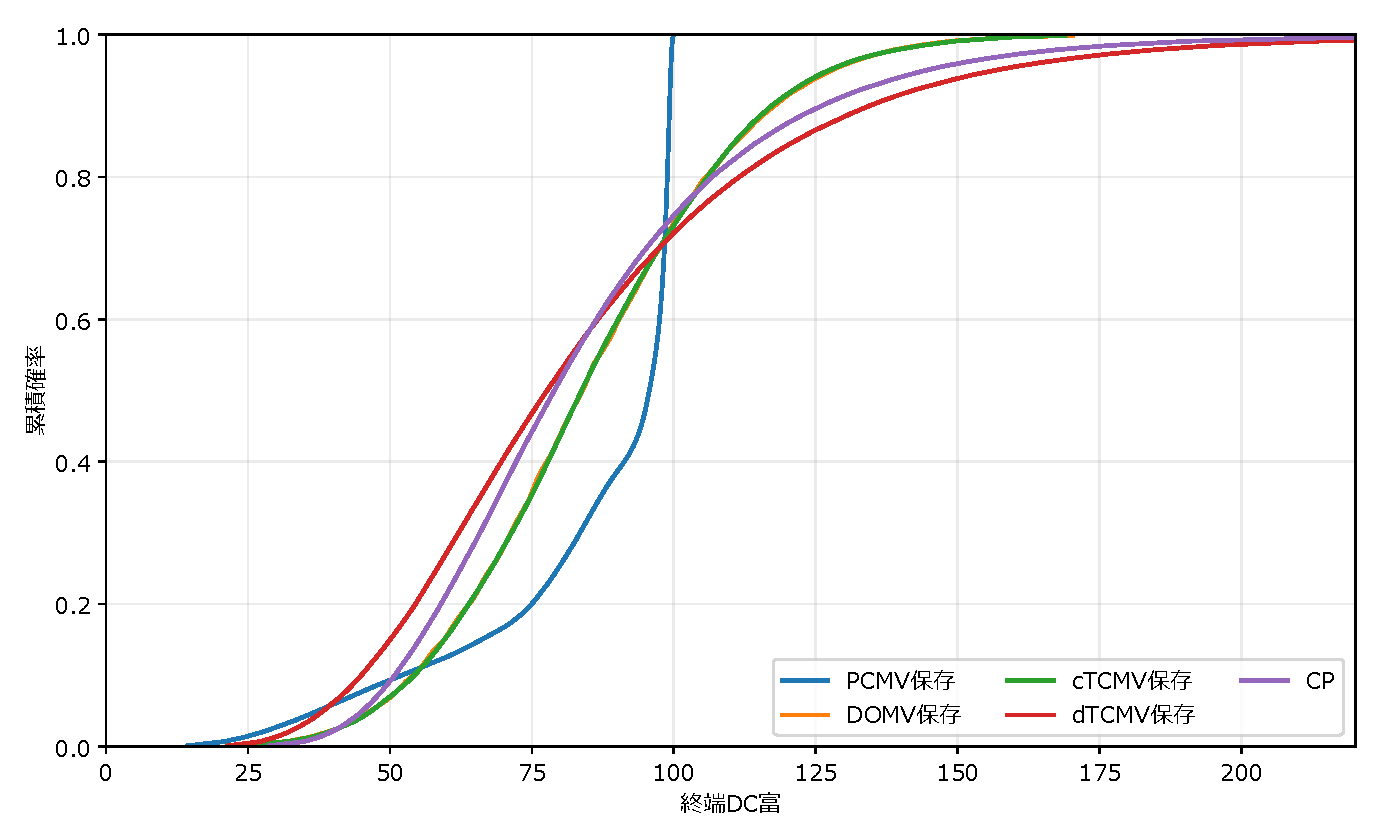
\includegraphics[width=.94\textwidth]{legacy_cdf.pdf}
\caption{旧保存方策の独立再評価による終価CDF．20万経路．共通平均の比較ではない．}\label{fig:cdf}
\end{figure}

図\ref{fig:cdf}は20万経路の経験分位点から描いた終端CDFである．曲線は保存方策の性能を示し，解析的な最適分布ではない．正規Euler再評価で300超を経験した割合はdTCMV保存方策で約0.137\%，CPで約0.030\%であった．小さい確率でも上位裾への寄与は無視できないため，dTCMVのUCVaRを高精度に確定したとは扱わない．全基準経路で負残高の切上げは発生しなかったが，発生確率が理論的にゼロであることは意味しない．

\subsection{同じ係数・固定ターゲットでのクリップ比較}
\begin{table}[htbp]\centering\small
\caption{クリップと保存方策の成果差：同一入力による診断}\label{tab:clip}
\begin{tabular}{lrrrr}
\toprule
解概念 & $G_{\mathrm{MAE}}$ & 平均差 & 平均差の95\%区間 & LCVaR差 \\ \midrule
PCMV & 0.030 & 1.654 & [1.634, 1.673] & -1.405 \\
DOMV & 0.086 & 3.748 & [3.715, 3.780] & -3.294 \\
cTCMV & 0.018 & -1.990 & [-2.005, -1.975] & 0.091 \\
dTCMV & 0.147 & 4.473 & [4.437, 4.508] & 0.952 \\
\bottomrule\end{tabular}
\par\vspace{3pt}\begin{minipage}{0.97\textwidth}\footnotesize 差はクリップ－保存方策．PCMVは固定ターゲット比較．dTCMVクリップには修正後の無制約係数を使用する．LCVaR差の信頼区間は推定していない．\end{minipage}
\end{table}
表\ref{tab:clip}の差は「クリップ－保存方策」である．各方策の平均差の信頼区間には，共通乱数による経路ごとの差の標準誤差を用いる．これにより，独立の標本同士を比較するより差を精密に推定できる．ただし，信頼区間は固定された方策・モデルのサンプリング誤差だけを表す．

PCMVとDOMVでは，この設定のクリップは平均を高める一方，LCVaRを下げる．cTCMVのクリップは平均を約1.99下げ，LCVaR差は約0.09にとどまる．平均配分差の小ささだけから，成果の近似が十分とは結論できない．

修正したdTCMVクリップでは，保存方策に比べ平均が約4.47高く，LCVaRも約0.95高い．したがって，従来の診断値を根拠に「dTCMVのクリップは下方裾を悪化させる」と一般化することはできない．この変化には無制約係数，評価方法および比較設定の修正が含まれ，符号変更だけの因果効果を識別したものでもない．保存方策を真の均衡とみなして，クリップが均衡を経済的に優越すると結論することもできない．


\begin{figure}[htbp]\centering
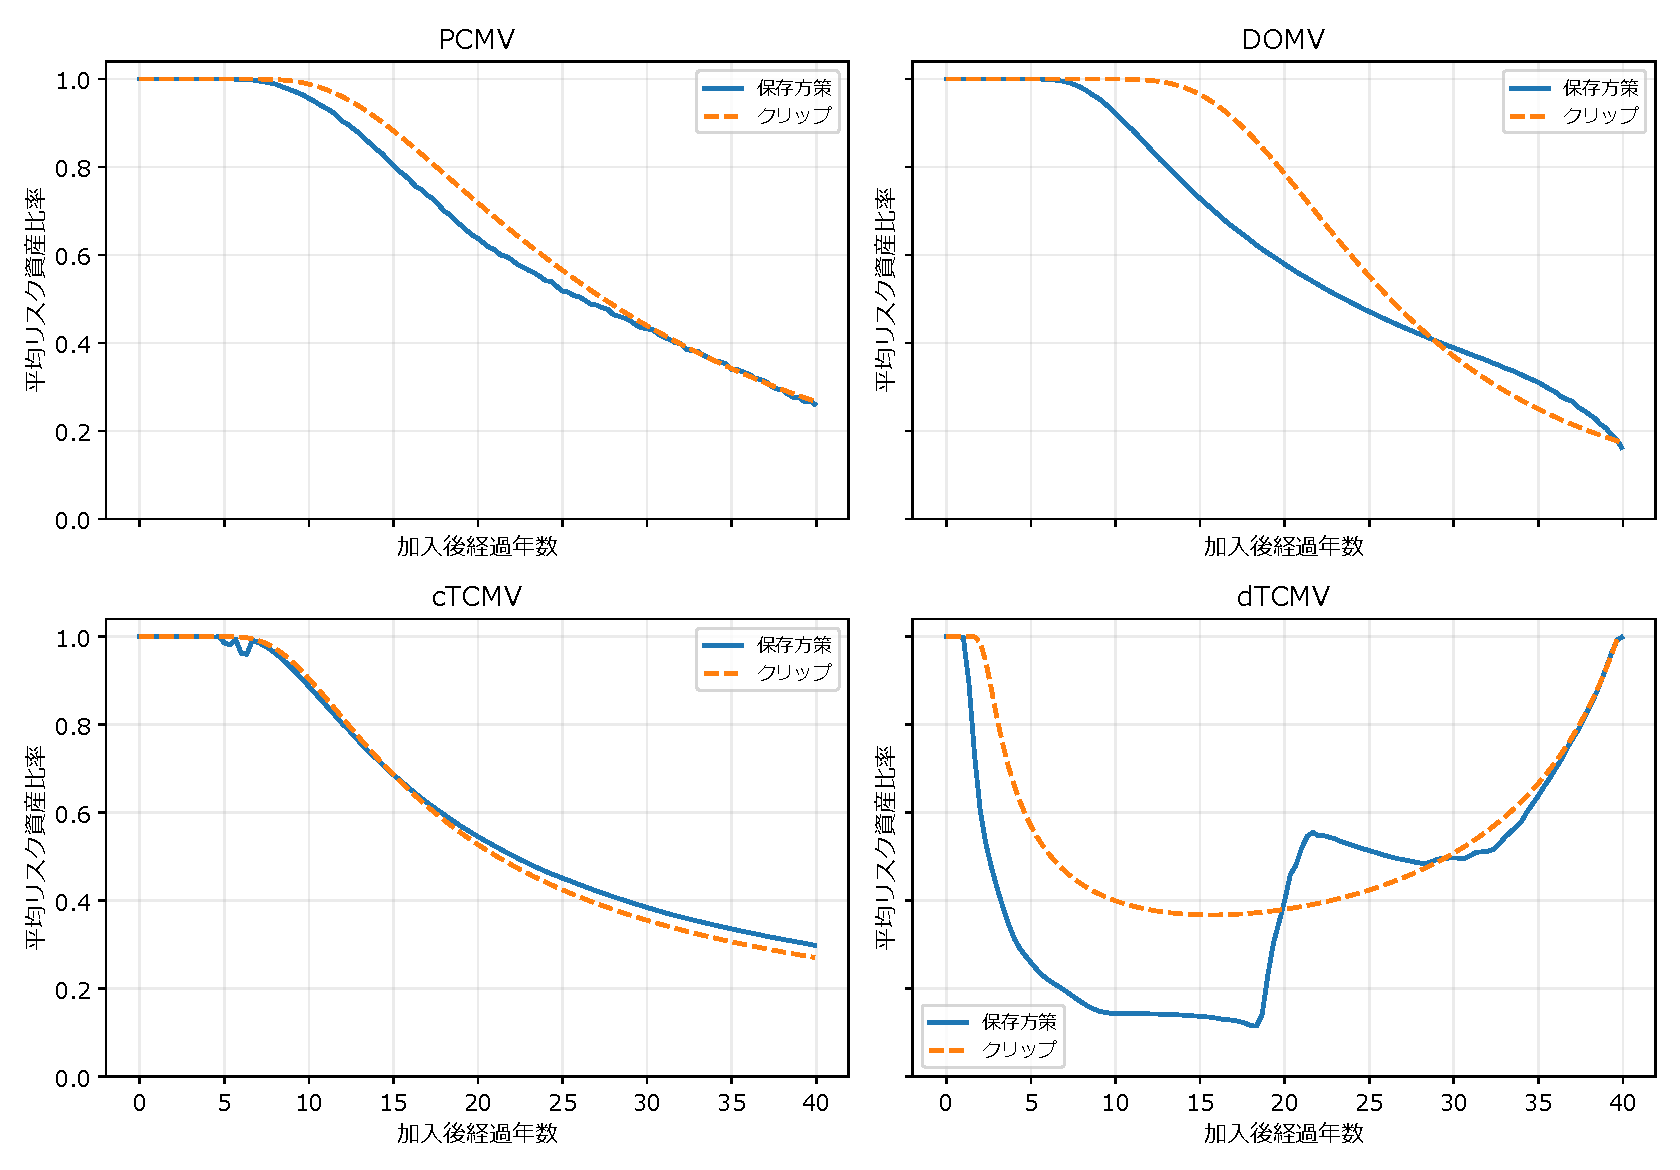
\includegraphics[width=.94\textwidth]{legacy_clipped.pdf}
\caption{旧保存方策とクリップの平均配分比較．同じ係数または固定ターゲットを使用．各方策自身の分布で平均した旧診断である．}\label{fig:glide}
\end{figure}

図\ref{fig:glide}は各方策自身の残高分布で平均した比率であり，一人の加入者の実現経路でも年齢だけの配分規則でもない．すべての曲線は最終意思決定時点$T-\Delta t$まで描き，未定義の終端制御をゼロで補完しない．

\subsection{補足監査と結果の位置づけ}
\begin{table}[htbp]\centering\small
\caption{格子配分のない三つの評価方法による標準偏差}\label{tab:robust}
\begin{tabular}{lrrr}
\toprule
方策 & 正規Euler & GH抽出Euler & 月次買持ち \\ \midrule
PCMV保存 & 19.77 & 19.76 & 19.73 \\
DOMV保存 & 24.71 & 24.67 & 24.86 \\
cTCMV保存 & 24.60 & 24.58 & 24.77 \\
dTCMV保存 & 38.20 & 38.27 & 38.47 \\
CP & 31.75 & 31.73 & 32.08 \\
\bottomrule\end{tabular}
\par\vspace{3pt}\begin{minipage}{0.97\textwidth}\footnotesize 正規Eulerは20万経路，他は各10万経路．すべて同じ保存方策・CP比率．月次買持ちは期末拠出を伴う別の運用仕様．\end{minipage}
\end{table}
表\ref{tab:robust}のGH抽出でも標準偏差は正規Eulerの再評価に近い．これは，参照格子との差をGH次数だけに帰する説明を支持しない．月次買持ちでも同様の水準だが，この近さをすべてのパラメータに一般化しない．ここでは各評価方法の乱数系列は独立比較として扱い，方法間の有意差検定は行っていない．

さらに，保存方策の継続モーメントを共通の上端集約モデルで計算し，命題\ref{prop:breakpoints}による一段階逸脱を調べた．到達確率と時点で平均した目的差はcTCMVで約$3.10\times10^{-4}$，dTCMVで約$1.53\times10^{-3}$であった．全格子上の最大差はそれぞれ7.24，5.02で，上端付近に現れた．全格子最大値と到達確率加重値は意味が異なる．また，参照後退ソルバーの上端線形外挿を本監査では集約へ統一しているため，これは元コードの同一目的上の残差をそのまま測った値ではない．境界仕様の相違を含めて，保存方策を\emph{共通の行確率遷移モデルの厳密な一段階均衡}と扱えないことを確認する監査である．

\FloatBarrier
\section{成果指標，誤差と再現手順}
\label{app:repro}
\subsection{分位点と下位・上位裾平均}
富の分布関数$F_W$に対し$q_\alpha=\inf\{w:F_W(w)\geq\alpha\}$と定義する．離散分布の場合，分位点上の質量を必要な割合だけ含め
\begin{align}
\mathrm{LCVaR}_\alpha&=\frac1\alpha\left\{\sum_{W_i<q_\alpha}p_iW_i+
\left(\alpha-\sum_{W_i<q_\alpha}p_i\right)q_\alpha\right\},\\
\mathrm{UCVaR}_\alpha&=\frac1\alpha\left\{\sum_{W_i>q_{1-\alpha}}p_iW_i+
\left(\alpha-\sum_{W_i>q_{1-\alpha}}p_i\right)q_{1-\alpha}\right\}.
\end{align}
本稿のLCVaRは損失のCVaRではなく下位富の平均なので，大きい方が下方成果は良い．経験分布の裾平均には下位・上位の所定数の経路を用いる．連続分位点の標本推定はNumPyの線形補間による．小数の桁数は精度保証ではない．

\subsection{尾部指標の誤差を監査する理由}
可積分な二分布の1次Wasserstein距離を$W_1=\int_0^1|q_u-\widetilde q_u|\dd u$とすると
\begin{equation}
|\E[W]-\E[\widetilde W]|\leq W_1,\qquad
|\mathrm{LCVaR}_\alpha(W)-\mathrm{LCVaR}_\alpha(\widetilde W)|\leq W_1/\alpha.
\end{equation}
分位関数の積分表示と三角不等式から従う．$\alpha=0.05$では同じ全体誤差の上界が20倍となるため，平均の一致だけで下位裾の精度は判断しない．この式は診断設計の根拠であり，本稿が参照分布と真の分布との$W_1$を既知として保証しているわけではない．

\subsection{参照版と今回の生成物}
参照コードと保存配列の公開元は
\begin{center}\url{https://github.com/yoshi123027-del/dc-glidepath-ica2026}\end{center}
であり，本稿の監査ではコミット\path{d02af6cf693ec701396c2ef8879c4b1b52e25b70}を固定した．監査対象は主として\path{results/monthly_D0_policy_arrays.npz}，\path{monthly_baseline_D0_summary.csv}，\path{equal_mean_calibration.csv}，ならびに後退・前進スクリプトである．参照版の基準CSVと本稿で新たに生成したCSVを混在させない．

再最適化は\path{recalibration/finite_model.py}，較正とDOMVターゲット群は\path{recalibration/run.py}，独立評価は\path{recalibration/validate.py}，前進一致・全境界監査は\path{recalibration/checks.py}で再現する．元の監査で用いた\path{audit.py}は，定率モーメント，無制約係数，保存方策とクリップの独立分布評価，状態別評価を実行する．\path{breakpoint_audit.py}は共通の上端集約核で一段階逸脱差を検査する．\path{verify_audit.py}は別の式による係数計算，CPの解析値との照合，確率・裾指標の整合性を検査する．本稿の同梱ファイルのSHA--256は\path{manifest_sha256.json}に記録する．

旧監査の主要設定は表\ref{tab:params}に示す．新方策の入力版はコミット\path{028a9ff9d4a41adb10495b2d05ff7191ac971121}の\path{results/recalibration_v8/fine/}である．本稿の追加評価は同梱\path{data/rolling_v9.csv}，\path{data/tail_intervals_v9.csv}に保存し，\path{README_JA.md}で再現手順を示す．掲載図は今回生成した数値から作成し，元PDFからの埋込み画像を数値の代替として使用しない．保存方策の外挿，乱数，GH重み，初期状態，負残高切上げの仕様をコードに明示する．

参照版の外部照合には，無制約特殊例を閉形式で再計算したものと，公表平均・標準偏差をアンカーとして対数正規分布を再構成したものが含まれる．後者はdTCMVの制御経路や係数の独立再現ではない．本稿では，この種の分布再構成を本稿の制約付きソルバー全体の検証証拠として使わない．

\section*{謝辞および開示}
生成AIを，原稿の編集，数式の検討，文献照合，検証コードの作成および図表生成の補助に使用した．本稿の再評価は実際に実行したコードの結果に基づく．理論・計算・引用および最終内容の確認と責任は著者が負う．本稿の数値例は特定の年金商品や加入者への投資助言を目的としない．

\begingroup\footnotesize\setlength{\bibsep}{1pt}\begin{thebibliography}{99}
\bibitem[Basak and Chabakauri(2010)]{BasakChabakauri2010}
Basak, S., and Chabakauri, G. (2010).
Dynamic mean--variance asset allocation.
\emph{Review of Financial Studies}, 23(8), 2970--3016.

\bibitem[Bjork et al.(2014)]{BjorkMurgociZhou2014}
Bjork, T., Murgoci, A., and Zhou, X. Y. (2014).
Mean--variance portfolio optimization with state-dependent risk aversion.
\emph{Mathematical Finance}, 24(1), 1--24.

\bibitem[Bjork et al.(2017)]{BjorkKhapkoMurgoci2017}
Bjork, T., Khapko, M., and Murgoci, A. (2017).
On time-inconsistent stochastic control in continuous time.
\emph{Finance and Stochastics}, 21, 331--360.

\bibitem[Bodie et al.(1992)]{BodieMertonSamuelson1992}
Bodie, Z., Merton, R. C., and Samuelson, W. F. (1992).
Labor supply flexibility and portfolio choice in a life-cycle model.
\emph{Journal of Economic Dynamics and Control}, 16(3--4), 427--449.

\bibitem[Cairns et al.(2006)]{CairnsBlakeDowd2006}
Cairns, A. J. G., Blake, D., and Dowd, K. (2006).
Stochastic lifestyling: Optimal dynamic asset allocation for defined contribution pension plans.
\emph{Journal of Economic Dynamics and Control}, 30(5), 843--877.

\bibitem[Falcone and Ferretti(2014)]{FalconeFerretti2014}
Falcone, M., and Ferretti, R. (2014).
\emph{Semi-Lagrangian Approximation Schemes for Linear and Hamilton--Jacobi Equations}.
SIAM.

\bibitem[Fleming and Soner(2006)]{FlemingSoner2006}
Fleming, W. H., and Soner, H. M. (2006).
\emph{Controlled Markov Processes and Viscosity Solutions}, 2nd ed.
Springer.

\bibitem[Haberman and Vigna(2002)]{HabermanVigna2002}
Haberman, S., and Vigna, E. (2002).
Optimal investment strategies and risk measures in defined contribution pension schemes.
\emph{Insurance: Mathematics and Economics}, 31(1), 35--69.
doi:10.1016/S0167-6687(02)00128-2.

\bibitem[Kushner and Dupuis(2001)]{KushnerDupuis2001}
Kushner, H. J., and Dupuis, P. G. (2001).
\emph{Numerical Methods for Stochastic Control Problems in Continuous Time}, 2nd ed.
Springer.

\bibitem[Li and Ng(2000)]{LiNg2000}
Li, D., and Ng, W.-L. (2000).
Optimal dynamic portfolio selection: Multiperiod mean--variance formulation.
\emph{Mathematical Finance}, 10(3), 387--406.

\bibitem[Menoncin and Vigna(2017)]{MenoncinVigna2017}
Menoncin, F., and Vigna, E. (2017).
Mean--variance target-based optimisation for defined contribution pension schemes in a stochastic framework.
\emph{Insurance: Mathematics and Economics}, 76, 172--184.
doi:10.1016/j.insmatheco.2017.08.002.

\bibitem[Menoncin and Vigna(2020)]{MenoncinVigna2020}
Menoncin, F., and Vigna, E. (2020).
Mean--variance dynamic optimality for DC pension schemes.
\emph{European Actuarial Journal}, 10, 125--148.
doi:10.1007/s13385-020-00226-1.

\bibitem[Merton(1969)]{Merton1969}
Merton, R. C. (1969).
Lifetime portfolio selection under uncertainty: The continuous-time case.
\emph{Review of Economics and Statistics}, 51(3), 247--257.

\bibitem[Pedersen and Peskir(2017)]{PedersenPeskir2017}
Pedersen, J. L., and Peskir, G. (2017).
Optimal mean--variance portfolio selection.
\emph{Mathematics and Financial Economics}, 11, 137--160.

\bibitem[van Staden et al.(2021)]{vanStadenDangForsyth2021}
van Staden, P. M., Dang, D.-M., and Forsyth, P. A. (2021).
On the distribution of terminal wealth under dynamic mean--variance optimal investment strategies.
\emph{SIAM Journal on Financial Mathematics}, 12(2), 566--603.
doi:10.1137/20M1338241.

\bibitem[Viceira(2001)]{Viceira2001}
Viceira, L. M. (2001).
Optimal portfolio choice for long-horizon investors with nontradable labor income.
\emph{Journal of Finance}, 56(2), 433--470.

\bibitem[Vigna and Haberman(2001)]{VignaHaberman2001}
Vigna, E., and Haberman, S. (2001).
Optimal investment strategy for defined contribution pension schemes.
\emph{Insurance: Mathematics and Economics}, 28(2), 233--262.
doi:10.1016/S0167-6687(00)00077-9.

\bibitem[Vigna(2014)]{Vigna2014}
Vigna, E. (2014).
On efficiency of mean--variance based portfolio selection in DC pension schemes.
\emph{Quantitative Finance}, 14(2), 237--258.
doi:10.1080/14697688.2012.708778.

\bibitem[Zhou and Li(2000)]{ZhouLi2000}
Zhou, X. Y., and Li, D. (2000).
Continuous-time mean--variance portfolio selection: A stochastic LQ framework.
\emph{Applied Mathematics and Optimization}, 42, 19--33.

\bibitem[ICA2026 Scientific Committee(2026a)]{ICA2026Guidance}
ICA2026 Scientific Committee (2026a).
\emph{Guidance for Preparing a Paper}.
\url{https://www.ica2026.org/doc/Guidance%20for%20Preparing%20a%20Paper.pdf}.
Accessed 11 September 2026.

\bibitem[ICA2026 Scientific Committee(2026b)]{ICA2026Call}
ICA2026 Scientific Committee (2026b).
\emph{Call for Papers}.
\url{https://www.ica2026.org/ab-submission.html}.
Accessed 11 September 2026.
\bibitem[Mu et al.(2019)]{MuTianYang2019}
Mu, C., Tian, W., and Yang, J. (2019).
Portfolio choice with skewness preference and wealth-dependent risk aversion.
\emph{Quantitative Finance}, 19(11), 1905--1919.
doi:10.1080/14697688.2019.1592214.


\bibitem[OECD(2025)]{OECD2025PensionMarkets}
OECD (2025).
\emph{Pension Markets in Focus 2025}.
Paris: OECD Publishing.
doi:10.1787/b095d0a0-en.


\end{thebibliography}\endgroup\end{document}